\documentclass[aspectratio=169]{beamer}

% 테마 설정
\usetheme{Madrid}
\usecolortheme{whale}

% 패키지
\usepackage{kotex}
\usepackage{amsmath}
\usepackage{amssymb}
\usepackage{graphicx}
\usepackage{booktabs}
\usepackage{tikz}
\usepackage{xcolor}
\usepackage{pifont}
\usepackage{multirow}
\usetikzlibrary{shapes,arrows,positioning,calc}

% 이미지 경로 설정
\graphicspath{{figures/}{figure/}}

% 수식 명령어
\DeclareMathOperator*{\argmin}{arg\,min}
\DeclareMathOperator*{\argmax}{arg\,max}

% 색상 정의
\definecolor{mainblue}{RGB}{0,82,147}
\definecolor{accentorange}{RGB}{230,126,34}
\definecolor{accentgreen}{RGB}{39,174,96}
\definecolor{lightgray}{RGB}{240,240,240}

% 프레임 번호 표시
\setbeamertemplate{footline}[frame number]

% 제목 정보
\title[MoLE-Flow]{MoLE-Flow: Mixture of LoRA Experts with \\ Normalizing Flow for Continual Anomaly Detection}
\subtitle{지속적 이상 탐지를 위한 LoRA 전문가 혼합 정규화 흐름}
\author{Hun Im, Pilsung Kang*}
\institute{Seoul National University}
\date{\today}

\begin{document}

%===============================================================================
% 제목 슬라이드
%===============================================================================

%-------------------------------------------------------------------------------
% Frame: Title Page
%-------------------------------------------------------------------------------
\begin{frame}
\titlepage
\end{frame}

%-------------------------------------------------------------------------------
% Frame: Contents
%-------------------------------------------------------------------------------
\begin{frame}{Contents}
\tableofcontents
\end{frame}

%===============================================================================
\section{Introduction}
%===============================================================================

%-------------------------------------------------------------------------------
% Frame: Problem - Continual Anomaly Detection
%-------------------------------------------------------------------------------
\begin{frame}{Problem: Continual Anomaly Detection}
\begin{columns}
\begin{column}{0.5\textwidth}
\textbf{산업 환경의 현실}
\begin{itemize}
    \item 새로운 제품이 지속적으로 추가됨
    \item 모든 데이터를 저장/재학습하기 어려움
    \item 이전 제품에 대한 성능 유지 필요
\end{itemize}

\vspace{1em}
\textbf{핵심 문제: Catastrophic Forgetting}
\begin{itemize}
    \item 새 작업 학습 시 이전 작업 성능 급감
    \item 기존 방법: 전체 모델 복제 $\rightarrow$ 메모리 비효율
\end{itemize}
\end{column}

\begin{column}{0.5\textwidth}
\centering
\begin{tikzpicture}[scale=0.8]
    % Task boxes
    \node[draw, fill=mainblue!20, minimum width=2cm, minimum height=1cm] (t0) at (0,2) {Task 0};
    \node[draw, fill=mainblue!30, minimum width=2cm, minimum height=1cm] (t1) at (0,0) {Task 1};
    \node[draw, fill=mainblue!40, minimum width=2cm, minimum height=1cm] (t2) at (0,-2) {Task 2};

    % Arrows
    \draw[->, thick] (t0) -- (t1);
    \draw[->, thick] (t1) -- (t2);

    % Performance indicator
    \node[draw, fill=red!30, minimum width=1.5cm] at (3.5,2) {100\%};
    \node[draw, fill=orange!30, minimum width=1.5cm] at (3.5,0) {70\%};
    \node[draw, fill=red!50, minimum width=1.5cm] at (3.5,-2) {40\%};

    \node at (3.5,3) {\small Task 0 성능};
\end{tikzpicture}   
\end{column}
\end{columns}
\end{frame}

%===============================================================================
\section{Previous Method}
%===============================================================================
% References:
% [ReplayCAD] Hu, Lei, et al. "ReplayCAD: Generative Diffusion Replay for Continual Anomaly Detection." arXiv preprint arXiv:2505.06603 (2025).
% [IUF] Tang, Jiaqi, et al. "An incremental unified framework for small defect inspection." ECCV 2024.
% [UCAD] Liu, Jiaqi, et al. "Unsupervised continual anomaly detection with contrastively-learned prompt." AAAI 2024.

%-------------------------------------------------------------------------------
% Frame: 기존 연구 방법
%-------------------------------------------------------------------------------
\begin{frame}{기존 연구 방법}
\begin{columns}
\begin{column}{0.33\textwidth}
\centering
\textbf{Replay 방식 (ReplayCAD)}
\vspace{0.3em}
\includegraphics[width=\textwidth]{replaycad.png}
\vspace{0.3em}
\small
이전 작업 데이터를 재사용하여 학습
\end{column}

\begin{column}{0.33\textwidth}
\centering
\textbf{Prompt 방식 (IUF)}
\vspace{0.3em}
\includegraphics[width=\textwidth]{iuf.png}
\vspace{0.3em}
\small
Class-specific 정보를 학습하기 위한 별도의 Discriminator를 사용
\end{column}

\begin{column}{0.33\textwidth}
\centering
\textbf{Adapter 방식 (UCAD)}
\vspace{0.3em}
\includegraphics[width=\textwidth]{ucad.png}
\vspace{0.3em}
\small
Class-specific 정보를 학습하기 위한 별도의 Prompt를 학습
\end{column}
\end{columns}

\vspace{1em}
\begin{alertblock}{기존 연구의 한계점}
\begin{itemize}
    \item \textbf{Replay 방식}: 오랜 학습 시간이 소요되며, replay로 인한 memory cost 존재
    \item \textbf{Adapter 방식}: Discriminator 또한 Catastrophic Forgetting 유발 가능성 있으며, 높은 학습 cost 존재
    \item \textbf{Prompt 방식}: 추론 단계에서 Task ID 인식을 위한 별도의 프로세스 필요
\end{itemize}
\end{alertblock}

\vfill
\tiny
\textcolor{gray}{[1] Hu et al., ReplayCAD, arXiv 2025 \quad [2] Tang et al., IUF, ECCV 2024 \quad [3] Liu et al., UCAD, AAAI 2024}
\end{frame}

%-------------------------------------------------------------------------------
% Frame: Our Solution - MoLE-Flow
%-------------------------------------------------------------------------------
\begin{frame}{Our Solution: MoLE-Flow}
    \begin{block}{핵심 아이디어: Parameter Isolation}
    Base 파라미터는 공유/고정하고, 경량 어댑터를 통해 만 task-specific 파라미터를 학습
    \end{block}

    \vspace{1em}
    \textbf{5가지 핵심 기여:}
    \begin{enumerate}
        \item \textcolor{mainblue}{\textbf{MoLE (Mixture of LoRA Experts)}}: NF coupling 블록에 LoRA 적용
        \item \textcolor{mainblue}{\textbf{WhiteningAdapter}}: 작업 간 분포 차이 정렬
        \item \textcolor{mainblue}{\textbf{Deep Invertible Adapter (DIA)}}: 비선형 매니폴드 적응
        \item \textcolor{mainblue}{\textbf{Prototype-based Router}}: Task ID 없이 자동 라우팅
        \item \textcolor{mainblue}{\textbf{Tail-Aware Loss}}: 분포 경계 학습 강화
    \end{enumerate}
    \end{frame}

%===============================================================================
\section{Overall Architecture}
%===============================================================================

%-------------------------------------------------------------------------------
% Frame: Overall Architecture
%-------------------------------------------------------------------------------
\begin{frame}{Overall Architecture}
\begin{center}
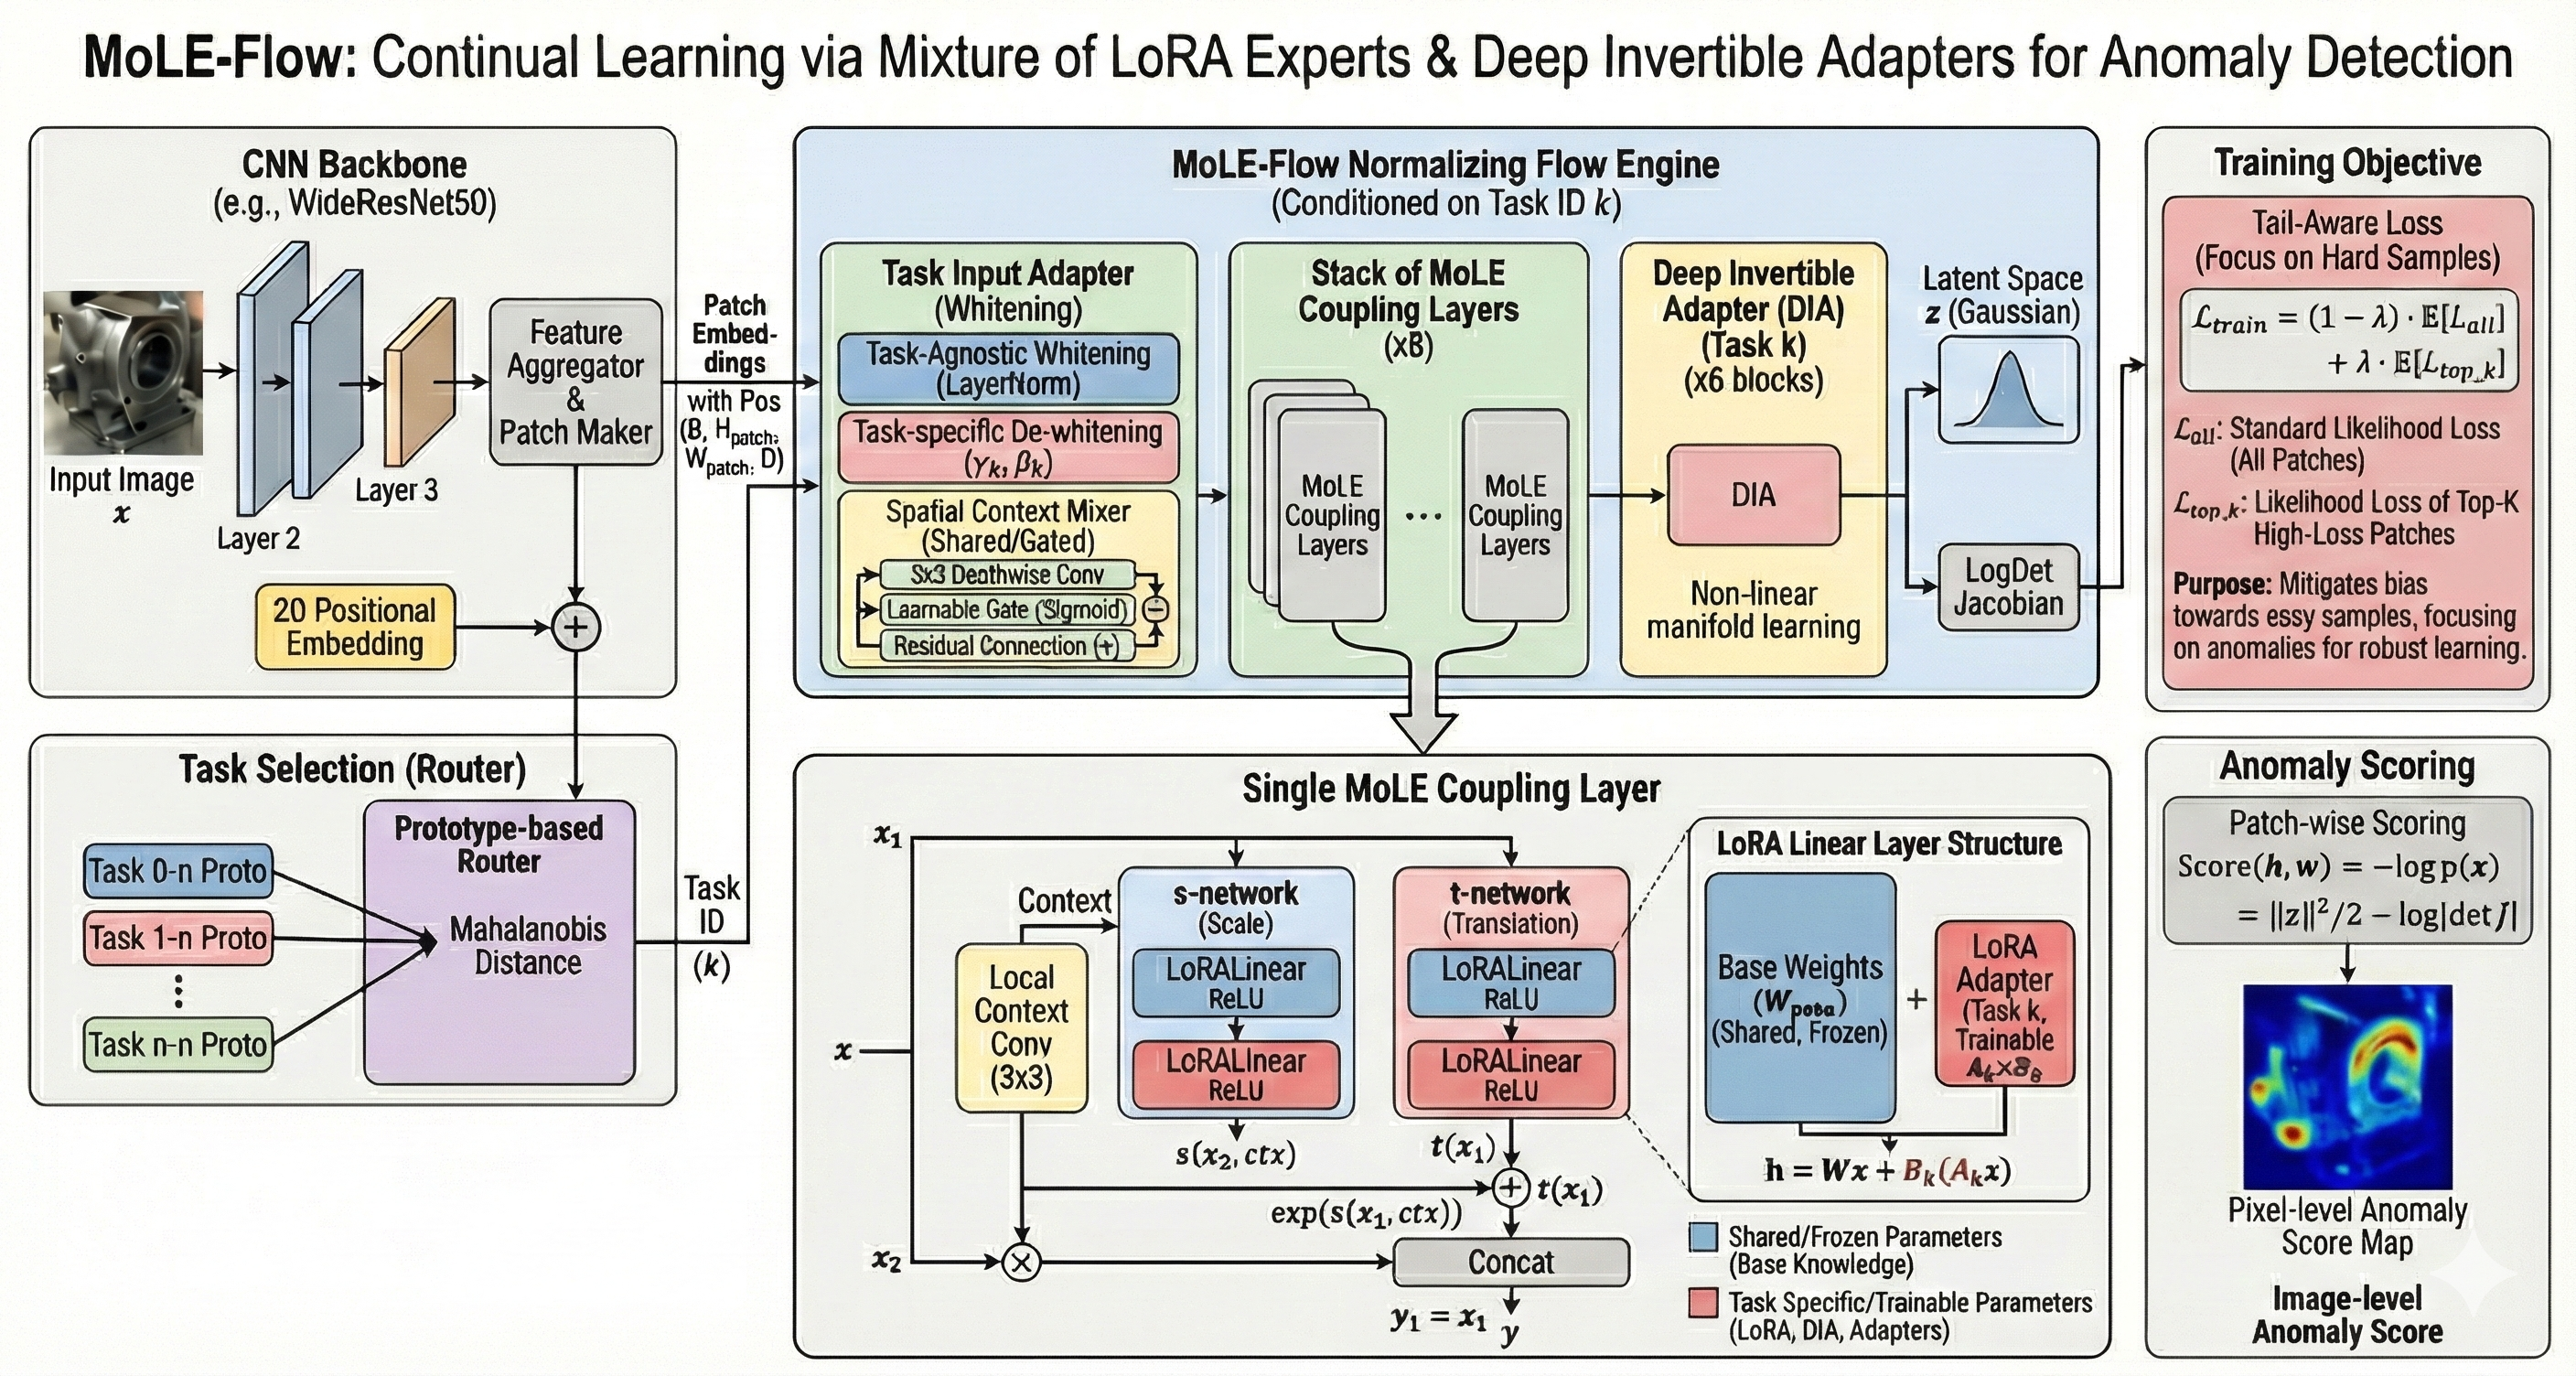
\includegraphics[width=0.95\textwidth]{figures/main2.png}
\end{center}
\end{frame}

%-------------------------------------------------------------------------------
% Frame: Overall Architecture - 학습 전략
%-------------------------------------------------------------------------------
\begin{frame}{Overall Architecture - 학습 전략}
\textbf{Parameter Isolation 전략:}
\begin{itemize}
    \item \textcolor{gray}{\textbf{회색 (Shared/Frozen)}}: Backbone, Base NF weights - 모든 작업이 공유
    \item \textcolor{red}{\textbf{빨간색 (Task-specific)}}: LoRA, DIA, Whitening Adapter - 작업별 독립
\end{itemize}

\vspace{1em}
\textbf{학습 전략:}
\begin{itemize}
    \item \textbf{Task 0}: Base NF + 모든 어댑터 학습 $\rightarrow$ Base 동결
    \item \textbf{Task $t > 0$}: 새로운 어댑터(LoRA, Whitening, DIA)만 학습
\end{itemize}

\vspace{1em}
\begin{alertblock}{핵심 장점}
작업당 \textbf{약 10.8\%}의 추가 파라미터만으로 완전한 작업 분리 달성
\end{alertblock}
\end{frame}

%-------------------------------------------------------------------------------
% Frame: Pipeline 수식
%-------------------------------------------------------------------------------
\begin{frame}{Pipeline 수식}
\begin{equation*}
\mathbf{x} \xrightarrow{\text{Backbone}} \mathbf{F} \xrightarrow{\text{PE}} \mathbf{F}' \xrightarrow{\text{Whitening}} \hat{\mathbf{F}} \xrightarrow{\text{SCM}} \tilde{\mathbf{F}} \xrightarrow{\text{NF+LoRA}} \mathbf{z}' \xrightarrow{\text{DIA}} (\mathbf{z}, \log|\det \mathbf{J}|)
\end{equation*}

\vspace{1em}
\begin{columns}
\begin{column}{0.5\textwidth}
\textbf{공유/고정 파라미터}
\begin{itemize}
    \item Backbone (ViT-Base)
    \item Base NF weights ($\mathbf{W}_{\text{base}}$)
    \item Spatial Context Mixer
\end{itemize}
\end{column}

\begin{column}{0.5\textwidth}
\textbf{Task-specific 파라미터}
\begin{itemize}
    \item LoRA: $\mathbf{A}_t, \mathbf{B}_t$
    \item Whitening: $\gamma_t, \beta_t$
    \item DIA: 별도 flow 블록
\end{itemize}
\end{column}
\end{columns}

\vspace{1em}
\begin{alertblock}{핵심 장점}
작업당 \textbf{약 10.8\%}의 추가 파라미터만으로 완전한 작업 분리 달성
\end{alertblock}
\end{frame}

%-------------------------------------------------------------------------------
% Frame: Notation
%-------------------------------------------------------------------------------
\begin{frame}{Notation: 주요 표기법}
\textbf{입력 및 특징}
\begin{itemize}
    \item $\mathbf{X} \in \mathbb{R}^{B \times H \times W \times D}$: 패치 임베딩 텐서 (배치 $B$, 공간 해상도 $H \times W$, 특징 차원 $D$)
    \item $\mathbf{x}_{u,v} \in \mathbb{R}^D$: 위치 $(u,v)$의 개별 패치 벡터
    \item $\mathbf{z}$: 잠재 공간 변수 (Normalizing Flow 출력)
\end{itemize}

\vspace{0.3em}
\textbf{작업 및 변환}
\begin{itemize}
    \item $t \in \{0, 1, \ldots, T-1\}$: 작업 인덱스
    \item $\mathbf{J}_f$: 함수 $f$의 Jacobian 행렬
    \item $\log|\det \mathbf{J}|$: Log-determinant (변환의 부피 변화율)
\end{itemize}

\vspace{0.3em}
\textbf{손실 함수 가중치}
\begin{itemize}
    \item $\lambda_{\text{tail}}$: Tail-Aware Loss 가중치 (default: 0.7)
    \item $\lambda_{\text{logdet}}$: Log-determinant 정규화 계수 (default: $10^{-4}$)
    \item $\lambda_{\text{reg}}$: 공분산 정규화 항 (default: $10^{-5}$)
\end{itemize}
\end{frame}

%-------------------------------------------------------------------------------
% Frame: Parameter Analysis (Backbone 제외)
%-------------------------------------------------------------------------------
\begin{frame}{Parameter Analysis (Backbone 제외)}
\textbf{Default Configuration:}
\scriptsize
\texttt{embed\_dim=512, coupling\_layers=8, lora\_rank=32, dia\_n\_blocks=4}

\vspace{0.5em}
\normalsize
\begin{columns}
\begin{column}{0.48\textwidth}
\textbf{Shared Parameters (Task 0 후 Freeze)}
\begin{table}
\scriptsize
\begin{tabular}{lr}
\toprule
\textbf{Module} & \textbf{Params} \\
\midrule
Base NF (8 subnets) & 5,255,168 \\
\quad s\_layer1 (512→512) & 2,101,248 \\
\quad s\_layer2 (512→256) & 1,050,624 \\
\quad t\_layer1 (256→512) & 1,052,672 \\
\quad t\_layer2 (512→256) & 1,050,624 \\
Context Conv (×8) & 40,968 \\
SpatialContextMixer & 5,121 \\
\midrule
\textbf{Total Shared} & \textbf{5,301,257} \\
\bottomrule
\end{tabular}
\end{table}
\end{column}

\begin{column}{0.48\textwidth}
\textbf{Per-Task Parameters (매 Task 생성)}
\begin{table}
\scriptsize
\begin{tabular}{lr}
\toprule
\textbf{Module} & \textbf{Params} \\
\midrule
LoRA Adapters (A+B) & 851,968 \\
\quad s\_layer1 LoRA & 262,144 \\
\quad s\_layer2 LoRA & 196,608 \\
\quad t\_layer1 LoRA & 196,608 \\
\quad t\_layer2 LoRA & 196,608 \\
Task Bias & 12,288 \\
WhiteningAdapter & 1,024 \\
DIA (4 blocks) & 1,579,008 \\
\midrule
\textbf{Total Per-Task} & \textbf{2,444,288} \\
\bottomrule
\end{tabular}
\end{table}
\end{column}
\end{columns}
\end{frame}

%-------------------------------------------------------------------------------
% Frame: Parameter Breakdown Visualization
%-------------------------------------------------------------------------------
\begin{frame}{Parameter Breakdown Visualization}
\begin{columns}
\begin{column}{0.55\textwidth}
\textbf{모듈별 파라미터 비중}

\vspace{0.5em}
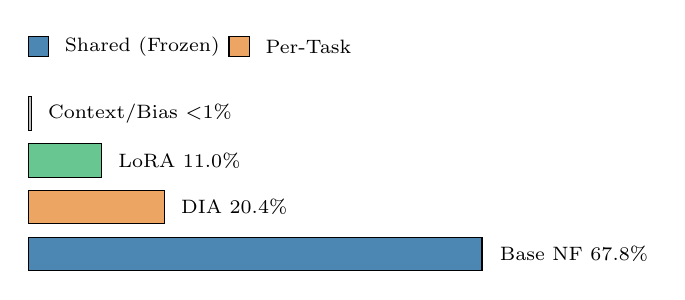
\begin{tikzpicture}[scale=0.85]
    % Bar chart
    \draw[fill=mainblue!70] (0,0) rectangle (6.78,0.5);
    \node[right] at (6.9,0.25) {\scriptsize Base NF 67.8\%};

    \draw[fill=accentorange!70] (0,0.7) rectangle (2.04,1.2);
    \node[right] at (2.14,0.95) {\scriptsize DIA 20.4\%};

    \draw[fill=accentgreen!70] (0,1.4) rectangle (1.1,1.9);
    \node[right] at (1.2,1.65) {\scriptsize LoRA 11.0\%};

    \draw[fill=gray!50] (0,2.1) rectangle (0.05,2.6);
    \node[right] at (0.15,2.35) {\scriptsize Context/Bias $<$1\%};

    % Legend
    \draw[fill=mainblue!70] (0,3.2) rectangle (0.3,3.5);
    \node[right] at (0.4,3.35) {\scriptsize Shared (Frozen)};

    \draw[fill=accentorange!70] (3,3.2) rectangle (3.3,3.5);
    \node[right] at (3.4,3.35) {\scriptsize Per-Task};
\end{tikzpicture}
\end{column}

\begin{column}{0.42\textwidth}
\textbf{Task 수에 따른 누적 파라미터}

\begin{table}
\scriptsize
\begin{tabular}{rrc}
\toprule
\textbf{Tasks} & \textbf{Total Params} & \textbf{증가량} \\
\midrule
Task 0 & 7.75M & - \\
Task 1 & 10.19M & +2.44M \\
Task 2 & 12.63M & +2.44M \\
Task 3 & 15.08M & +2.44M \\
\midrule
\textbf{15 Tasks} & \textbf{41.97M} & - \\
\bottomrule
\end{tabular}
\end{table}

\vspace{0.5em}
\begin{alertblock}{\scriptsize Per-Task 비율}
\scriptsize
$\frac{2.44\text{M}}{7.75\text{M}} \approx \textbf{31.6\%}$ (Task 0 대비) \\
Backbone (86M) 제외 시 매우 효율적
\end{alertblock}
\end{column}
\end{columns}
\end{frame}

%-------------------------------------------------------------------------------
% Frame: Parameter Distribution (Pie Chart)
%-------------------------------------------------------------------------------
\begin{frame}{Parameter Distribution (Per-Task 기준)}
\begin{columns}
\begin{column}{0.5\textwidth}
\centering
\textbf{Per-Task 파라미터 구성}

\vspace{0.5em}
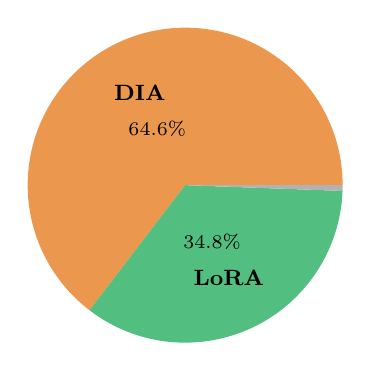
\begin{tikzpicture}[scale=1.0]
    % Pie chart for Per-Task parameters
    % DIA: 64.6%, LoRA: 34.8%, Bias: 0.5%, Whitening: 0.04%

    % DIA slice (64.6% = 232.6 degrees)
    \fill[accentorange!80] (0,0) -- (0:2) arc (0:232.6:2) -- cycle;
    \node at (116.3:1.3) {\footnotesize \textbf{DIA}};
    \node at (116.3:0.8) {\scriptsize 64.6\%};

    % LoRA slice (34.8% = 125.3 degrees)
    \fill[accentgreen!80] (0,0) -- (232.6:2) arc (232.6:357.9:2) -- cycle;
    \node at (295.3:1.3) {\footnotesize \textbf{LoRA}};
    \node at (295.3:0.8) {\scriptsize 34.8\%};

    % Task Bias + Whitening (0.6%)
    \fill[gray!60] (0,0) -- (357.9:2) arc (357.9:360:2) -- cycle;

\end{tikzpicture}

\vspace{0.3em}
\scriptsize
\textcolor{gray}{Task Bias + Whitening $<$ 1\%}
\end{column}

\begin{column}{0.5\textwidth}
\centering
\textbf{전체 모델 파라미터 구성 (Task 0)}

\vspace{0.5em}
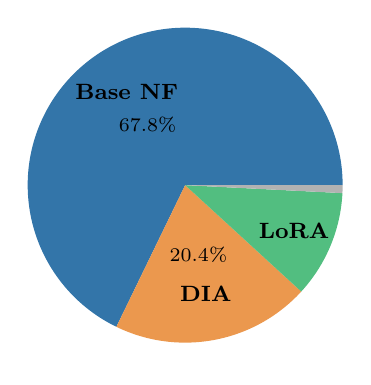
\begin{tikzpicture}[scale=1.0]
    % Total: 7.75M
    % Base NF: 67.8% = 244.1 degrees
    % DIA: 20.4% = 73.4 degrees
    % LoRA: 11.0% = 39.6 degrees
    % Others: 0.8% = 2.9 degrees

    % Base NF (Shared)
    \fill[mainblue!80] (0,0) -- (0:2) arc (0:244.1:2) -- cycle;
    \node at (122:1.4) {\footnotesize \textbf{Base NF}};
    \node at (122:0.9) {\scriptsize 67.8\%};

    % DIA
    \fill[accentorange!80] (0,0) -- (244.1:2) arc (244.1:317.5:2) -- cycle;
    \node at (280.8:1.4) {\footnotesize \textbf{DIA}};
    \node at (280.8:0.9) {\scriptsize 20.4\%};

    % LoRA
    \fill[accentgreen!80] (0,0) -- (317.5:2) arc (317.5:357.1:2) -- cycle;
    \node at (337.3:1.5) {\footnotesize \textbf{LoRA}};

    % Others
    \fill[gray!60] (0,0) -- (357.1:2) arc (357.1:360:2) -- cycle;

\end{tikzpicture}

\vspace{0.3em}
\scriptsize
\textcolor{mainblue!80}{■} Shared (Frozen) \quad
\textcolor{accentorange!80}{■} \textcolor{accentgreen!80}{■} Per-Task
\end{column}
\end{columns}
\end{frame}

%-------------------------------------------------------------------------------
% Frame: Cumulative Parameters Graph
%-------------------------------------------------------------------------------
\begin{frame}{Task 수에 따른 누적 파라미터 증가}
\begin{center}
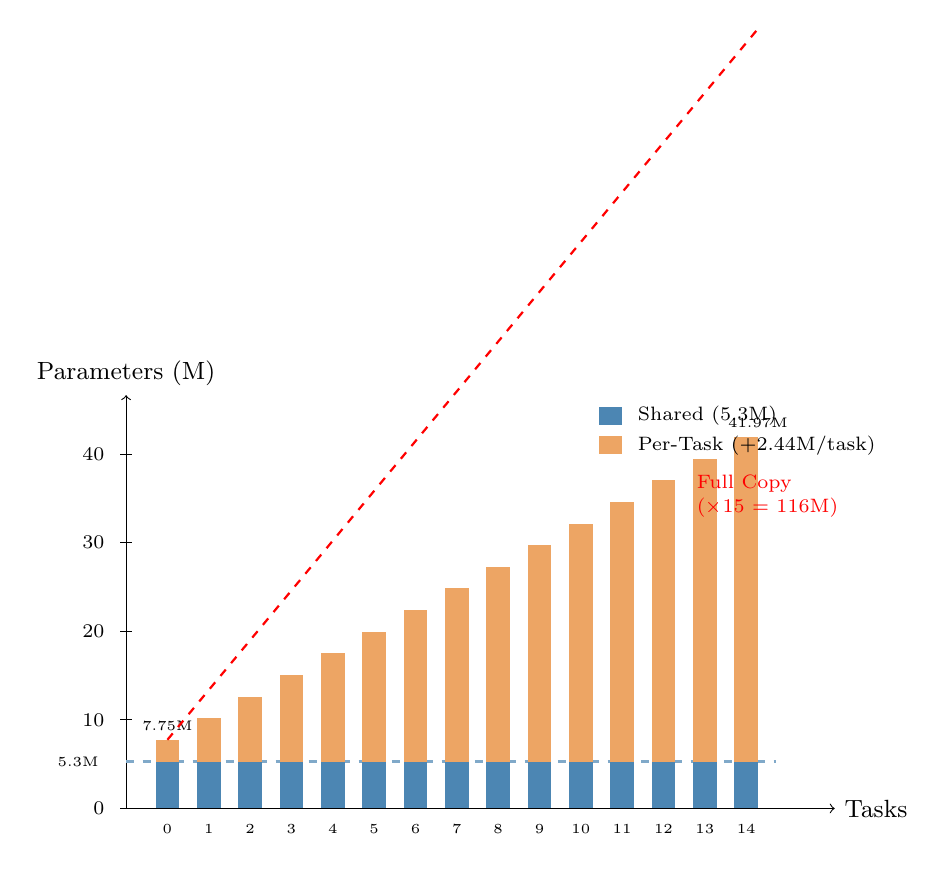
\begin{tikzpicture}[scale=0.75]
    % Axes
    \draw[->] (0,0) -- (12,0) node[right] {\small Tasks};
    \draw[->] (0,0) -- (0,7) node[above] {\small Parameters (M)};

    % Y-axis labels
    \foreach \y/\label in {0/0, 1.5/10, 3/20, 4.5/30, 6/40} {
        \draw (-0.1,\y) -- (0.1,\y);
        \node[left] at (-0.2,\y) {\scriptsize \label};
    }

    % X-axis labels
    \foreach \x/\label in {0.7/0, 1.4/1, 2.1/2, 2.8/3, 3.5/4, 4.2/5, 4.9/6, 5.6/7, 6.3/8, 7/9, 7.7/10, 8.4/11, 9.1/12, 9.8/13, 10.5/14} {
        \node[below] at (\x,-0.1) {\tiny \label};
    }

    % Shared base (horizontal line at 5.3M = 0.795)
    \draw[dashed, mainblue!50, thick] (0,0.795) -- (11,0.795);
    \node[left] at (-0.3,0.795) {\tiny 5.3M};

    % Per-task stacked bars
    % Task 0: 7.75M total (5.3M shared + 2.44M per-task)
    \fill[mainblue!70] (0.5,0) rectangle (0.9,0.795);
    \fill[accentorange!70] (0.5,0.795) rectangle (0.9,1.163);

    % Task 1-14: cumulative
    \foreach \t/\h in {1/1.529, 2/1.895, 3/2.261, 4/2.627, 5/2.993, 6/3.359, 7/3.725, 8/4.091, 9/4.457, 10/4.823, 11/5.189, 12/5.555, 13/5.921, 14/6.287} {
        \pgfmathsetmacro{\x}{0.5 + \t*0.7}
        \fill[mainblue!70] (\x,0) rectangle (\x+0.4,0.795);
        \fill[accentorange!70] (\x,0.795) rectangle (\x+0.4,\h);
    }

    % Labels
    \node[above] at (0.7,1.163) {\tiny 7.75M};
    \node[above] at (10.7,6.287) {\tiny 41.97M};

    % Legend
    \fill[mainblue!70] (8,6.5) rectangle (8.4,6.8);
    \node[right] at (8.5,6.65) {\scriptsize Shared (5.3M)};
    \fill[accentorange!70] (8,6) rectangle (8.4,6.3);
    \node[right] at (8.5,6.15) {\scriptsize Per-Task (+2.44M/task)};

    % Comparison line for full model duplication
    \draw[red, dashed, thick] (0.7,1.163) -- (10.7,6.287*2.1);
    \node[red, right] at (9.5,5.5) {\scriptsize Full Copy};
    \node[red, right] at (9.5,5.1) {\scriptsize (×15 = 116M)};

\end{tikzpicture}
\end{center}

\begin{alertblock}{효율성 비교}
\textbf{MoLE-Flow}: 15 Tasks에서 \textbf{41.97M} 파라미터 \\
\textbf{Full Model Copy}: 15 Tasks에서 \textbf{116.25M} 파라미터 → \textbf{64\% 절약}
\end{alertblock}
\end{frame}

%-------------------------------------------------------------------------------
% Frame: DIA Parameter Details
%-------------------------------------------------------------------------------
\begin{frame}{DIA (Deep Invertible Adapter) Parameter Details}
\textbf{DIA 구조: 4개의 AffineCouplingBlock}

\vspace{0.5em}
\begin{columns}
\begin{column}{0.5\textwidth}
\textbf{AffineCouplingBlock 구성}
\begin{itemize}
    \item \texttt{split\_dim = 512 / 2 = 256}
    \item \texttt{hidden\_dim = 512 × 0.5 = 256}
\end{itemize}

\vspace{0.5em}
\textbf{SimpleSubnet (s\_net, t\_net)}
\begin{itemize}
    \item Linear(256 → 256): 65,792
    \item Linear(256 → 256): 65,792
    \item Linear(256 → 256): 65,792
    \item \textbf{Subnet Total}: 197,376
\end{itemize}
\end{column}

\begin{column}{0.5\textwidth}
\textbf{파라미터 계산}
\begin{table}
\scriptsize
\begin{tabular}{lr}
\toprule
\textbf{Component} & \textbf{Params} \\
\midrule
s\_net (per block) & 197,376 \\
t\_net (per block) & 197,376 \\
\midrule
\textbf{Block Total} & 394,752 \\
\midrule
\textbf{4 Blocks Total} & \textbf{1,579,008} \\
\bottomrule
\end{tabular}
\end{table}

\vspace{0.5em}
\begin{block}{\scriptsize DIA의 역할}
\scriptsize
비선형 매니폴드 적응으로 \\
LoRA가 표현 못하는 복잡한 분포 변환 학습
\end{block}
\end{column}
\end{columns}
\end{frame}

%===============================================================================
\section{Feature Extraction}
%===============================================================================

%-------------------------------------------------------------------------------
% Frame: Feature Extraction & Preprocessing
%-------------------------------------------------------------------------------
\begin{frame}{Feature Extraction \& Preprocessing}
\begin{columns}
\begin{column}{0.6\textwidth}
\textbf{1. Backbone (ViT-Base)}
\begin{itemize}
    \item 사전 학습된 ViT 사용 (Frozen)
    \item 다중 스케일 특징: 블록 $\{1, 3, 5, 11\}$
\end{itemize}

\vspace{0.5em}
\textbf{2. Patch Maker}
\begin{itemize}
    \item Feature Map을 패치 단위로 분할
    \item 출력: $\mathbf{F} \in \mathbb{R}^{B \times H \times W \times D}$
    \item PatchCore의 방식과 동일하게 패치 단위로 분할하여 패치 임베딩을 생성
\end{itemize}

\vspace{0.5em}
\textbf{3. Positional Encoding}
\begin{itemize}
    \item NF의 순열 불변성 극복
    \item 2D Sinusoidal PE 추가
\end{itemize}
\begin{equation*}
\mathbf{F}' = \mathbf{F} + \mathbf{P}
\end{equation*}
\end{column}

\begin{column}{0.4\textwidth}
\centering
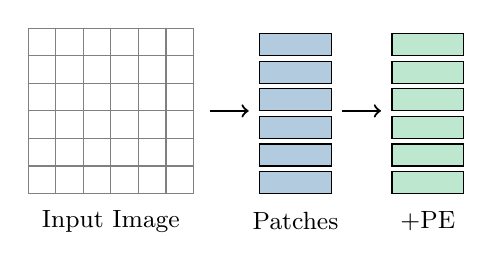
\begin{tikzpicture}[scale=0.7]
    % Image grid
    \draw[step=0.5cm, gray, thin] (0,0) grid (3,3);
    \node at (1.5,-0.5) {\small Input Image};

    % Arrow
    \draw[->, thick] (3.3,1.5) -- (4,1.5);

    % Patch embeddings
    \foreach \y in {0,0.5,1,1.5,2,2.5} {
        \draw[fill=mainblue!30] (4.2,\y) rectangle (5.5,\y+0.4);
    }
    \node at (4.85,-0.5) {\small Patches};

    % Arrow
    \draw[->, thick] (5.7,1.5) -- (6.4,1.5);

    % PE added
    \foreach \y in {0,0.5,1,1.5,2,2.5} {
        \draw[fill=accentgreen!30] (6.6,\y) rectangle (7.9,\y+0.4);
    }
    \node at (7.25,-0.5) {\small +PE};
\end{tikzpicture}
\end{column}
\end{columns}
\end{frame}

%-------------------------------------------------------------------------------
% Frame: Feature Extraction - Why Positional Encoding?
%-------------------------------------------------------------------------------
\begin{frame}{Why Positional Encoding?}
\textbf{Normalizing Flow의 구조적 특성:}
\begin{itemize}
    \item NF는 입력을 1D 벡터로 평탄화하여 처리
    \item 각 패치 임베딩이 \textbf{독립적}으로 처리됨 (Permutation Invariance)
    \item 패치의 \textbf{공간적 위치 정보가 소실}
\end{itemize}

\vspace{0.5em}
\textbf{Positional Encoding 적용:}
\begin{equation*}
\mathbf{F}' = \mathbf{F} + \mathbf{P}, \quad \mathbf{P} \in \mathbb{R}^{H \times W \times D}
\end{equation*}

\vspace{0.3em}
\begin{columns}[T]
\begin{column}{0.48\textwidth}
\textbf{2D Sinusoidal PE}
\begin{itemize}
    \item 행과 열에 대해 독립적인 주파수 사용
    \item 연속적인 위치 관계 표현
    \item 학습 파라미터 없음
\end{itemize}
\end{column}

\begin{column}{0.48\textwidth}
\textbf{효과}
\begin{itemize}
    \item 동일한 특징이라도 위치에 따라 다르게 처리
    \item 이상치의 ``어디''가 중요한지 인식
    \item 공간적 패턴 학습 가능
\end{itemize}
\end{column}
\end{columns}

\vspace{0.3em}
\begin{block}{핵심}
NF는 ``무엇(What)''만 처리 $\rightarrow$ PE 추가로 ``어디(Where)'' 정보 주입 $\rightarrow$ 위치 기반 이상 탐지
\end{block}
\end{frame}

%===============================================================================
\section{Task Adapters}
%===============================================================================

%-------------------------------------------------------------------------------
% Frame: Task Adapters - Whitening
%-------------------------------------------------------------------------------
\begin{frame}{Task Adapters: WhiteningAdapter}
\textbf{\textcolor{red}{문제}: 클래스별 이미지 분포 차이}
\begin{itemize}
    \item 클래스별로 다른 이미지 통계량 $\rightarrow$ NF 학습 불안정
    \item Task 전환 시 급격한 입력 분포 변화 (Covariate Shift)
    \item 고정된 Base Flow가 새로운 분포에 최적 반응 불가
\end{itemize}

\vspace{0.3em}
\textbf{\textcolor{accentgreen}{해결}: 2단계 Whitening 전략}

\vspace{0.3em}
\begin{columns}[T]
\begin{column}{0.48\textwidth}
\textbf{Step 1: Task-Agnostic Whitening}
\begin{equation*}
\mathbf{x}_{\text{white}} = \frac{\mathbf{F}' - \mathbb{E}[\mathbf{F}']}{\sqrt{\text{Var}[\mathbf{F}'] + \epsilon}}
\end{equation*}
\begin{itemize}
    \item 모든 Task를 \textbf{동일한 시작점}으로
    \item LayerNorm 기반 (학습 파라미터 없음)
    \item 분포 스케일 차이 사전 제거
\end{itemize}
\end{column}
\begin{column}{0.48\textwidth}
\textbf{Step 2: Task-Specific De-whitening}
\begin{equation*}
\hat{\mathbf{F}}_t = \gamma_t \odot \mathbf{x}_{\text{white}} + \beta_t
\end{equation*}
\begin{itemize}
    \item $\gamma_t$: 채널별 중요도 조절
    \item $\beta_t$: Base Flow 최적 영역으로 이동
    \item \textbf{범위 제한}으로 안정성 확보
\end{itemize}
\end{column}
\end{columns}

\vspace{0.3em}
\begin{block}{핵심 원리: Affine 변환을 사용하는 이유}
\small 통계적 특성(평균, 분산)만 조절하고 데이터의 본질적 구조(Shape)는 보존 $\rightarrow$ FiLM~\cite{perez2018film}과 유사
\end{block}
\end{frame}

%-------------------------------------------------------------------------------
% Frame: WhiteningAdapter - Why Affine Transformation (상세)
%-------------------------------------------------------------------------------
\begin{frame}{WhiteningAdapter: Why Affine Transformation?}
\textbf{De-whitening에서 Affine 변환 ($\mathbf{y} = \gamma \odot \mathbf{x} + \beta$)을 사용하는 이유:}

\vspace{0.3em}
\begin{columns}[T]
\begin{column}{0.48\textwidth}
\textbf{1. 통계적 정합성}
\begin{itemize}
    \item 정규분포 $\rightarrow$ 정규분포 변환의 자연스러운 방법
    \item $\mathcal{N}(0,1) \rightarrow \mathcal{N}(\mu_t, \sigma_t^2)$
    \item 비선형 변환 시 분포 모양 왜곡 (Bell curve 소실)
\end{itemize}

\vspace{0.3em}
\textbf{2. 구조 보존}
\begin{itemize}
    \item 공간 늘림(Scale) + 이동(Shift)만 수행
    \item 직선$\rightarrow$직선, 평행선$\rightarrow$평행선 유지
    \item 데이터 ``내용(Content)'' 보존
\end{itemize}
\end{column}

\begin{column}{0.48\textwidth}
\textbf{3. 역할 분담}
\begin{itemize}
    \item Adapter: 1차/2차 모멘트(평균, 분산) 정렬
    \item Base Flow + LoRA: 복잡한 비선형 분포 모델링
    \item BatchNorm~\cite{ioffe2015batchnorm}의 $\gamma$, $\beta$와 동일 원리
\end{itemize}

\vspace{0.3em}
\textbf{4. 채널별 중요도 조절}
\begin{itemize}
    \item $\gamma_t \uparrow$: 해당 특징 증폭
    \item $\gamma_t \downarrow$: 해당 특징 억제
    \item 예: 가죽$\rightarrow$질감 채널 증폭, 나사$\rightarrow$형태 채널 증폭
\end{itemize}
\end{column}
\end{columns}

\vspace{0.3em}
\begin{alertblock}{De-whitening의 본질}
단순 원래 분포 복원이 아닌, \textbf{고정된 Base Flow의 매니폴드 상에서 각 Task 데이터가 최적으로 표현될 위치 학습}
\end{alertblock}
\end{frame}

%===============================================================================
\section{MoLE-Flow}
%===============================================================================

% Development Journey frame removed - content moved to Experiments Part 1: Optimization Journey

%-------------------------------------------------------------------------------
% Frame: MoLE-Flow - Spatial Context Mixer
%-------------------------------------------------------------------------------
\begin{frame}{MoLE-Flow: Spatial Context Mixer}
\begin{columns}[T]
\begin{column}{0.55\textwidth}
\centering
\includegraphics[width=\textwidth]{spatial_context_mixer.png}
\end{column}

\begin{column}{0.42\textwidth}
\textbf{\textcolor{red}{문제}: 패치 독립 처리의 한계}
\begin{itemize}
    \item 기존 NF: $p(\mathbf{X}) \approx \prod_{u,v} p(\mathbf{x}_{u,v})$
    \item 주변 맥락 정보 부족
    \item 결함 경계(Local Contrast) 인식 어려움
\end{itemize}

\vspace{0.3em}
\textbf{\textcolor{accentgreen}{해결}: Gated Depthwise Aggregation}
\begin{equation*}
\mathbf{x}_{\text{mixed}} = (1-g) \cdot \mathbf{x} + g \cdot \mathbf{x}_{\text{ctx}}
\end{equation*}

\vspace{0.2em}
\small
\begin{itemize}
    \item $\mathbf{x}_{\text{ctx}}$: DepthwiseConv$_{K\times K}$
    \item $g = \sigma(\theta)$: 학습 가능 게이트
    \item 채널 독립적 공간 집계
\end{itemize}
\end{column}
\end{columns}

\vspace{0.3em}
\begin{block}{핵심 원리: Pseudo-Dependency Modeling}
\small NF 구조 변경 없이 $\mathbf{z}_{u,v}$가 이웃 정보 $\mathcal{N}_{u,v}$를 내포 $\rightarrow$ 간접적 조건부 확률 $p(\mathbf{x}_{u,v}|\mathcal{N}_{u,v})$ 학습
\end{block}
\end{frame}

%-------------------------------------------------------------------------------
% Frame: MoLE-Flow - LoRA-based Coupling Layer
%-------------------------------------------------------------------------------
\begin{frame}{MoLE-Flow: LoRA-based Coupling Layer}
\textbf{\textcolor{red}{문제}: 전체 모델 Fine-tuning의 한계}
\begin{itemize}
    \item 전체 파라미터 학습 $\rightarrow$ \textbf{Catastrophic Forgetting} 발생
    \item Task별 별도 모델 저장 $\rightarrow$ 메모리 비효율
\end{itemize}

\vspace{0.5em}
\begin{center}
\includegraphics[width=0.75\textwidth]{Molesubnet.png}
\end{center}

\vspace{0.3em}
\textbf{\textcolor{accentgreen}{해결}: LoRA (Low-Rank Adaptation)}
\begin{equation*}
\mathbf{h}(\mathbf{x}) = \underbrace{\mathbf{W}_{\text{base}}\mathbf{x}}_{\text{Base (Frozen)}} + \underbrace{\frac{\alpha}{r}(\mathbf{B}\mathbf{A})\mathbf{x}}_{\text{LoRA (Task-specific)}} + (\mathbf{b}_{\text{base}} + \mathbf{b}_t)
\end{equation*}

\textbf{\textcolor{mainblue}{효과}}: Task당 \textbf{약 2.1M} 파라미터 ($\sim$11\% of total)
\end{frame}

%-------------------------------------------------------------------------------
% Frame: MoLE-Flow - LoRA-based Coupling Layer (상세)
%-------------------------------------------------------------------------------
\begin{frame}{MoLE-Flow: LoRA-based Coupling Layer (상세)}
\begin{columns}
\begin{column}{0.5\textwidth}
\textbf{Base Linear (Frozen Anchor)}
\begin{itemize}
    \item Task 0에서 학습 후 \textbf{영구 고정}
    \item 범용적인 특징 변환 역할
    \item 모든 작업이 공유하는 ``공통 지식''
\end{itemize}

\vspace{0.5em}
\textbf{Why Frozen?}
\begin{itemize}
    \item 새 Task 학습 시 Base 변경 $\rightarrow$ 이전 Task 성능 저하
    \item Parameter Isolation의 핵심 원리
\end{itemize}
\end{column}

\begin{column}{0.5\textwidth}
\textbf{LoRA Linear (Task-Specialist)}
\begin{itemize}
    \item 작업 고유 분포 특성 보정
    \item 저랭크 행렬: $\Delta\mathbf{W} = \mathbf{B}\mathbf{A}$
    \item 작업마다 독립적인 $\mathbf{A}_t, \mathbf{B}_t$ 생성
\end{itemize}

\vspace{0.5em}
\textbf{초기화 전략:}
\begin{itemize}
    \item $\mathbf{A}$: Xavier uniform (다양성)
    \item $\mathbf{B}$: Zero $\rightarrow$ 학습 시작 시 $\Delta\mathbf{W}=0$
    \item Base에서 점진적으로 분기
\end{itemize}
\end{column}
\end{columns}

\vspace{0.5em}
\begin{block}{핵심 원리: Parameter Isolation}
\small Base(공유) + LoRA(분리) 구조로 작업 간 간섭을 \textbf{원천 차단} $\rightarrow$ Forgetting $\approx$ 0
\end{block}
\end{frame}

%-------------------------------------------------------------------------------
% Frame: MoLE-Flow - Context-Aware s/t Networks
%-------------------------------------------------------------------------------
\begin{frame}{MoLE-Flow: Scale Context (s-network only)}
\textbf{\textcolor{red}{문제}: s-network가 anomaly 판단에 주변 정보 필요}
\begin{itemize}
    \item 이상치의 ``크기(scale)''는 주변 패치와의 \textbf{상대적 비교}에 의존
    \item t-network는 분포 중심 이동만 담당 $\rightarrow$ context 불필요
\end{itemize}

\vspace{0.5em}
\textbf{\textcolor{accentgreen}{해결}: s-network에만 Context 입력}

\vspace{0.5em}
\begin{columns}
\begin{column}{0.5\textwidth}
\textbf{Scale Network (Context-Aware)}
\begin{equation*}
\mathbf{s} = f_s([\mathbf{x}; \mathbf{ctx}_{K \times K}])
\end{equation*}
\begin{itemize}
    \item 원본 + $K \times K$ 문맥 정보 결합
    \item 이상치 ``돌출'' 정도 판단
    \item DepthwiseConv로 효율적 집계
\end{itemize}
\end{column}

\begin{column}{0.5\textwidth}
\textbf{Translation Network (Context-Free)}
\begin{equation*}
\mathbf{t} = f_t(\mathbf{x})
\end{equation*}
\begin{itemize}
    \item 원본 특징만 사용
    \item 분포 중심은 패치 고유 특성
    \item Context 추가 시 오히려 노이즈
\end{itemize}
\end{column}
\end{columns}

\vspace{0.5em}
\begin{block}{핵심 원리: 역할 분리}
\small Scale $\mathbf{s}$: 주변 대비 ``얼마나 다른가'' (상대적) / Translation $\mathbf{t}$: ``어디로 이동할지'' (절대적)
\end{block}
\end{frame}

%-------------------------------------------------------------------------------
% Frame: MoLEContextSubnet Architecture (상세)
%-------------------------------------------------------------------------------
\begin{frame}{MoLEContextSubnet: Context-Aware \& Task-Adaptive Design}
\textbf{Coupling Layer 내부 핵심 모듈: 변환 파라미터 ($\mathbf{s}$, $\mathbf{t}$) 생성}

\vspace{0.3em}
\textbf{1. Spatial Structure Recovery \& Context Extraction}
\begin{itemize}
    \item 일반 NF: 1D 벡터 평탄화 $\rightarrow$ 공간적 인접성 소실
    \item 본 모듈: 2D 이미지 재구성 후 $3 \times 3$ DepthwiseConv로 문맥 추출
    \item 게이팅 적용: $\mathbf{ctx} = \alpha \cdot \mathbf{c}(\mathbf{x})$, where $\alpha = \alpha_{\max} \cdot \sigma(\theta_{\text{scale}})$
\end{itemize}

\vspace{0.3em}
\textbf{2. 비대칭 네트워크 설계}
\begin{columns}[T]
\begin{column}{0.48\textwidth}
\textbf{Context-Aware s-network}
\begin{equation*}
\mathbf{s} = \text{MLP}([\mathbf{x}; \mathbf{ctx}])
\end{equation*}
\begin{itemize}
    \item 결함 = 주변과의 \textbf{불연속성}
    \item 국소적 대비(Local Contrast) 포착
\end{itemize}
\end{column}
\begin{column}{0.48\textwidth}
\textbf{Context-Free t-network}
\begin{equation*}
\mathbf{t} = \text{MLP}(\mathbf{x})
\end{equation*}
\begin{itemize}
    \item 분포 중심 이동은 패치 고유 특성
    \item 문맥 추가 시 불필요한 간섭
\end{itemize}
\end{column}
\end{columns}

\vspace{0.3em}
\begin{block}{가역성 보장}
LoRA는 subnet 내부 선형 레이어에만 적용 $\rightarrow$ Coupling 구조의 가역성에 영향 없음 \\
\small $\mathbf{y} = [\mathbf{x}_1, \mathbf{x}_2 \odot \exp(\mathbf{s}) + \mathbf{t}] \Leftrightarrow \mathbf{x} = [\mathbf{y}_1, (\mathbf{y}_2 - \mathbf{t}) \odot \exp(-\mathbf{s})]$
\end{block}
\end{frame}

%-------------------------------------------------------------------------------
% Frame: Hierarchical Context Processing
%-------------------------------------------------------------------------------
\begin{frame}{Hierarchical Context Processing: 문맥 모듈 비교}
\textbf{Spatial Context Mixer vs MoLEContextSubnet 내부 Context Conditioning}

\vspace{0.5em}
\begin{columns}[T]
\begin{column}{0.48\textwidth}
\textbf{Spatial Context Mixer}
\begin{itemize}
    \item \textbf{위치}: Flow 입력 \textbf{이전}
    \item \textbf{역할}: ``이 패치가 어떤 이웃을 가지는가''를 특징 자체에 인코딩
    \item \textbf{성격}: \textbf{전처리} 모듈
\end{itemize}
\end{column}

\begin{column}{0.48\textwidth}
\textbf{MoLEContextSubnet Context}
\begin{itemize}
    \item \textbf{위치}: 각 Coupling Layer \textbf{내부}
    \item \textbf{역할}: ``이 이웃 관계에서 어떤 스케일 변화가 적절한가'' 결정
    \item \textbf{성격}: \textbf{변환 가이드}
\end{itemize}
\end{column}
\end{columns}

\vspace{0.5em}
\begin{center}
\begin{tikzpicture}[scale=0.85]
    \node[draw, fill=blue!10, minimum width=2.8cm, minimum height=0.7cm] (scm) at (0,0) {\scriptsize Spatial Context Mixer};
    \node[below=0.05cm of scm, font=\tiny] {입력 수준 문맥 인코딩};

    \node[draw, fill=orange!10, minimum width=2.8cm, minimum height=0.7cm] (mole) at (5,0) {\scriptsize MoLEContextSubnet};
    \node[below=0.05cm of mole, font=\tiny] {변환 수준 적응적 스케일링};

    \draw[->, thick] (scm) -- node[above, font=\tiny] {보완적 작용} (mole);
\end{tikzpicture}
\end{center}

\vspace{0.3em}
\begin{alertblock}{두 모듈이 모두 필요한 이유}
입력 수준 문맥 인코딩 + 변환 수준 적응적 스케일링 = \textbf{계층적 문맥 처리 (Hierarchical Context Processing)}
\end{alertblock}
\end{frame}

%-------------------------------------------------------------------------------
% Frame: MoLE-Flow - Deep Invertible Adapter (DIA)
%-------------------------------------------------------------------------------
\begin{frame}{MoLE-Flow: Deep Invertible Adapter (DIA)}
\textbf{\textcolor{red}{문제}: 선형 변환의 표현력 한계}
\begin{itemize}
    \item LoRA: $\mathbf{W} + \mathbf{BA}$ $\rightarrow$ 선형 변환
    \item WhiteningAdapter: $\gamma \cdot \mathbf{x} + \beta$ $\rightarrow$ 선형 변환
    \item 복잡한 \textbf{비선형 매니폴드 차이} 보상 어려움
\end{itemize}

\vspace{0.5em}
\textbf{\textcolor{accentgreen}{해결}: DIA (Deep Invertible Adapter)}
\begin{equation*}
\mathbf{z}_{\text{final}} = f_{\text{DIA}}^{(t)}(\mathbf{z}_{\text{base}}), \quad \text{with } \log|\det \mathbf{J}_{\text{DIA}}|
\end{equation*}

\vspace{0.3em}
\begin{columns}
\begin{column}{0.55\textwidth}
\textbf{DIA 구조:}
\begin{itemize}
    \item AffineCouplingBlock 스택
    \item Task별 독립 파라미터
    \item \textbf{Near-identity 초기화}: $f_{\text{DIA}}(\mathbf{z}) \approx \mathbf{z}$
\end{itemize}
\end{column}
\begin{column}{0.42\textwidth}
\textbf{Why Invertible?}
\begin{itemize}
    \item NF의 밀도 추정 속성 보존
    \item Jacobian 계산 가능
    \item 학습 안정성 향상
\end{itemize}
\end{column}
\end{columns}

\vspace{0.3em}
\begin{block}{핵심 원리: 비선형 매니폴드 적응}
\small LoRA(선형)가 표현 못하는 복잡한 분포 변환 학습. Base Flow 출력을 Task별 최적 잠재 공간으로 비선형 매핑
\end{block}
\end{frame}

%-------------------------------------------------------------------------------
% Frame: DIA - AffineCouplingBlock (상세)
%-------------------------------------------------------------------------------
\begin{frame}{DIA: AffineCouplingBlock 상세 구조}
\textbf{각 AffineCouplingBlock의 변환 과정:}

\vspace{0.3em}
\begin{enumerate}
    \item \textbf{Split}: $[\mathbf{x}_1, \mathbf{x}_2] = \text{Split}(\mathbf{x})$ (채널 절반 분할)
    \item \textbf{Subnet}: $\mathbf{s}, \mathbf{t} = \text{SimpleSubnet}(\mathbf{x}_1)$ (scale, translation 예측)
    \item \textbf{Soft-Clamping}: $\tilde{\mathbf{s}} = \alpha_{\text{clamp}} \cdot \tanh(\mathbf{s}/\alpha_{\text{clamp}})$ (수치 안정성)
    \item \textbf{Transform}: $\mathbf{y}_2 = \mathbf{x}_2 \odot \exp(\tilde{\mathbf{s}}) + \mathbf{t}$
    \item \textbf{Concat}: $\mathbf{y} = \text{Concat}(\mathbf{x}_1, \mathbf{y}_2)$
\end{enumerate}

\vspace{0.3em}
\textbf{Log-Determinant 계산}
\begin{equation*}
\log|\det \mathbf{J}_{\text{block}}| = \sum_{i=1}^{D/2} \tilde{s}_i = \sum_{i=1}^{D/2} \alpha_{\text{clamp}} \cdot \tanh(s_i/\alpha_{\text{clamp}})
\end{equation*}

\vspace{0.3em}
\begin{alertblock}{MoLEContextSubnet vs DIA 역할 차이}
\begin{itemize}
    \item \textbf{MoLEContextSubnet}: ``공간 인지형 범용 변환기'' - Base anchor + LoRA로 범용 변환 + 작업별 적응
    \item \textbf{DIA}: ``작업 특화 분포 보정기'' - 완전히 독립적인 파라미터로 정밀 분포 보정
\end{itemize}
\end{alertblock}
\end{frame}

%-------------------------------------------------------------------------------
% Frame: DIA vs MoLEContextSubnet - Why Different Design?
%-------------------------------------------------------------------------------
\begin{frame}{DIA가 Spatial Context를 사용하지 않는 이유}
\textbf{MoLEContextSubnet과 DIA는 모두 Affine Coupling 기반이지만 다른 설계 철학}

\vspace{0.5em}
\begin{columns}[T]
\begin{column}{0.48\textwidth}
\textbf{MoLEContextSubnet}
\begin{itemize}
    \item ``공간 인지형 범용 변환기''
    \item Base weights를 anchor로 범용 변환 보존
    \item LoRA로 작업별 적응
    \item Spatial context로 국소 이상 패턴에 민감
    \item ``정상 $\rightarrow$ 표준 정규분포'' 변환의 뼈대
\end{itemize}
\end{column}

\begin{column}{0.48\textwidth}
\textbf{DIA}
\begin{itemize}
    \item ``작업 특화 분포 보정기''
    \item Task별 완전 독립 파라미터
    \item Spatial context \textbf{불사용}:
    \begin{enumerate}
        \scriptsize
        \item 잠재 공간에서 동작 - 공간 정보는 이미 MoLEContextSubnet에서 인코딩
        \item 역할 분리: 공간 인지 변환 vs 분포 정밀 보정
        \item 파라미터 오버헤드 최소화
    \end{enumerate}
\end{itemize}
\end{column}
\end{columns}

\vspace{0.3em}
\begin{block}{핵심 설계 원리}
MoLEContextSubnet이 ``공간 인지 변환''을, DIA가 ``분포 정밀 보정''을 담당하는 \textbf{명확한 역할 분리}가 효율적
\end{block}
\end{frame}

% Key Insights and Trade-offs frames removed - content moved to Experiments Part 1

%===============================================================================
\section{Training \& Inference}
%===============================================================================

%-------------------------------------------------------------------------------
% Frame: Training Objective - Likelihood Calculation
%-------------------------------------------------------------------------------
\begin{frame}{Training Objective: Likelihood Calculation}
\textbf{Normalizing Flow의 핵심: 변수 변환}
\begin{equation*}
\log p(\mathbf{x}) = \log p(\mathbf{z}_{\text{final}}) + \log|\det \mathbf{J}_{\text{total}}|
\end{equation*}

\vspace{1em}
\begin{columns}
\begin{column}{0.5\textwidth}
\textbf{잠재 확률}
\begin{equation*}
\log p(\mathbf{z}) = -\frac{1}{2}\|\mathbf{z}\|_2^2 - \frac{D}{2}\log(2\pi)
\end{equation*}
\begin{itemize}
    \item 표준 정규분포 가정
    \item 원점에 가까울수록 높은 확률
\end{itemize}
\end{column}

\begin{column}{0.5\textwidth}
\textbf{Jacobian 누적}
\begin{equation*}
\log|\det \mathbf{J}_{\text{total}}| = \log|\det \mathbf{J}_{\text{flow}}| + \log|\det \mathbf{J}_{\text{DIA}}|
\end{equation*}
\begin{itemize}
    \item 각 변환의 부피 변화율
    \item 밀도 보정 역할
\end{itemize}
\end{column}
\end{columns}
\end{frame}

%-------------------------------------------------------------------------------
% Frame: Training Objective - Tail-Aware Loss
%-------------------------------------------------------------------------------
\begin{frame}{Training Objective: Tail-Aware Loss}
\textbf{\textcolor{red}{문제}: 일반 NLL의 한계}
\begin{itemize}
    \item 모든 패치의 평균 NLL 최소화
    \item ``쉬운'' 정상 패치에만 집중 $\rightarrow$ \textbf{경계 학습 부족}
    \item 정상/이상 경계의 ``어려운'' 패치 무시
\end{itemize}

\vspace{0.5em}
\textbf{\textcolor{accentgreen}{해결}: Tail-Aware Loss}
\begin{equation*}
\mathcal{L}_{\text{train}} = (1 - \lambda) \cdot \mathbb{E}[\mathcal{L}_{\text{all}}] + \lambda \cdot \mathbb{E}[\mathcal{L}_{\text{top-k}}]
\end{equation*}

\begin{columns}
\begin{column}{0.5\textwidth}
\textbf{핵심 아이디어:}
\begin{itemize}
    \item $\mathcal{L}_{\text{top-k}}$: 상위 k\% 고손실 패치
    \item 분포 경계(tail)에 위치한 ``어려운'' 샘플 집중 학습
\end{itemize}
\end{column}
\begin{column}{0.48\textwidth}
\textbf{Why Tail?}
\begin{itemize}
    \item Anomaly는 정상 분포의 ``꼬리''에 위치
    \item 경계 패치 학습 $\rightarrow$ 분리 능력 향상
    \item Hard negative mining과 유사 개념
\end{itemize}
\end{column}
\end{columns}

\vspace{0.3em}
\begin{block}{핵심 원리: 분포 경계 학습 강화}
\small 쉬운 패치만 학습하면 경계가 불명확 $\rightarrow$ Tail 패치 가중치로 결정 경계 선명화
\end{block}
\end{frame}

%-------------------------------------------------------------------------------
% Frame: Training Objective - LogDet Regularization
%-------------------------------------------------------------------------------
\begin{frame}{Training Objective: LogDet Regularization}
\textbf{\textcolor{red}{문제}: Jacobian 불안정성}
\begin{itemize}
    \item NF의 log-determinant가 불안정 $\rightarrow$ density estimation 품질 저하
    \item Deep NF에서 Jacobian explosion/vanishing 문제 발생
    \item 변환의 volume 변화가 극단적 $\rightarrow$ 밀도 추정 왜곡
\end{itemize}

\vspace{0.5em}
\textbf{\textcolor{accentgreen}{해결}: LogDet Regularization}
\begin{equation*}
\mathcal{L}_{\text{total}} = \mathcal{L}_{\text{NLL}} + \lambda_{\text{logdet}} \cdot |\log|\det \mathbf{J}||
\end{equation*}

\vspace{0.5em}
\begin{columns}
\begin{column}{0.5\textwidth}
\textbf{핵심 아이디어:}
\begin{itemize}
    \item $|\log|\det \mathbf{J}|| \rightarrow 0$ 유도
    \item Volume-preserving 변환
    \item 학습 안정성 향상
\end{itemize}
\end{column}
\begin{column}{0.48\textwidth}
\textbf{Why Log-Det?}
\begin{itemize}
    \item $\log|\det \mathbf{J}| = 0$ $\Leftrightarrow$ 부피 보존
    \item 극단적 축소/확대 방지
    \item Invertibility 보장 강화
\end{itemize}
\end{column}
\end{columns}

\vspace{0.3em}
\begin{block}{핵심 원리: 변환의 부피 보존}
\small Log-determinant를 0 근처로 정규화 $\rightarrow$ 변환이 정보를 압축/팽창하지 않고 형태만 변형
\end{block}
\end{frame}

%-------------------------------------------------------------------------------
% Frame: Inference - Task Routing
%-------------------------------------------------------------------------------
\begin{frame}{Inference: Task Routing}
\textbf{핵심 문제: 추론 시 Task ID가 주어지지 않음}

\vspace{1em}
\textbf{해결: Prototype-based Mahalanobis Router}
\begin{equation*}
t^* = \argmin_t D_M(\mathbf{f}, t), \quad D_M(\mathbf{f}, t) = \sqrt{(\mathbf{f} - \boldsymbol{\mu}_t)^\top \boldsymbol{\Sigma}_t^{-1} (\mathbf{f} - \boldsymbol{\mu}_t)}
\end{equation*}

\vspace{0.5em}
\textbf{장점:}
\begin{itemize}
    \item \textbf{One-stage}: 별도의 라우팅 추론 불필요
    \item \textbf{공분산 고려}: 분포 형태를 반영한 거리 측정
    \item \textbf{스케일 불변}: 특징 차원 간 스케일 차이 자동 보정
\end{itemize}

\begin{alertblock}{기존 방법 대비 장점}
기존: Two-stage (라우팅 $\rightarrow$ 탐지) \\
Ours: \textbf{One-stage} (라우팅 + 탐지 동시)
\end{alertblock}
\end{frame}

%-------------------------------------------------------------------------------
% Frame: Task Routing - Prototype Construction (상세)
%-------------------------------------------------------------------------------
\begin{frame}{Task Routing: Prototype Construction (상세)}
\textbf{Training Phase에서 각 Task의 Prototype 구축}

\vspace{0.5em}
\begin{columns}[T]
\begin{column}{0.55\textwidth}
\textbf{Prototype 구성 요소}
\begin{itemize}
    \item 평균 벡터 $\boldsymbol{\mu}_t \in \mathbb{R}^D$
    \item 공분산 행렬 $\boldsymbol{\Sigma}_t \in \mathbb{R}^{D \times D}$
\end{itemize}

\vspace{0.3em}
\textbf{계산 방법}
\begin{align*}
\boldsymbol{\mu}_t &= \frac{1}{N_t} \sum_{i=1}^{N_t} \mathbf{f}_i^{(t)} \\
\boldsymbol{\Sigma}_t &= \frac{1}{N_t - 1} \sum_{i=1}^{N_t} (\mathbf{f}_i^{(t)} - \boldsymbol{\mu}_t)(\mathbf{f}_i^{(t)} - \boldsymbol{\mu}_t)^\top + \lambda_{\text{reg}} \mathbf{I}
\end{align*}
\end{column}

\begin{column}{0.42\textwidth}
\textbf{특징 벡터 $\mathbf{f}$}
\begin{itemize}
    \item Backbone 마지막 layer 출력
    \item 이미지 레벨 특징 벡터
    \item $\mathbf{f}_{\text{backbone}} \in \mathbb{R}^D$
\end{itemize}

\vspace{0.3em}
\textbf{Precision Matrix}
\begin{itemize}
    \item $\boldsymbol{\Sigma}_t^{-1}$ 사전 계산
    \item $\lambda_{\text{reg}} = 10^{-5}$ (수치 안정성)
\end{itemize}
\end{column}
\end{columns}

\vspace{0.3em}
\begin{block}{Adapter 활성화}
선택된 Task $t^*$에 따라: \textbf{LoRA} $\{\mathbf{A}_{t^*}, \mathbf{B}_{t^*}\}$ + \textbf{Whitening} $\{\boldsymbol{\mu}_{t^*}^{\text{white}}, \boldsymbol{\sigma}_{t^*}^{\text{white}}\}$ + \textbf{DIA} 활성화
\end{block}
\end{frame}

%-------------------------------------------------------------------------------
% Frame: Why Mahalanobis Distance?
%-------------------------------------------------------------------------------
\begin{frame}{Why Mahalanobis Distance?}
\textbf{Euclidean vs Mahalanobis 거리 비교}

\vspace{0.5em}
\begin{columns}[T]
\begin{column}{0.48\textwidth}
\textbf{Euclidean Distance}
\begin{equation*}
D_E(\mathbf{f}, t) = \|\mathbf{f} - \boldsymbol{\mu}_t\|_2
\end{equation*}
\begin{itemize}
    \item 모든 방향을 \textbf{동등하게} 취급
    \item 특징 차원 간 스케일 차이 무시
    \item 분포 형태 미반영
\end{itemize}
\end{column}

\begin{column}{0.48\textwidth}
\textbf{Mahalanobis Distance}
\begin{equation*}
D_M(\mathbf{f}, t) = \sqrt{(\mathbf{f} - \boldsymbol{\mu}_t)^\top \boldsymbol{\Sigma}_t^{-1} (\mathbf{f} - \boldsymbol{\mu}_t)}
\end{equation*}
\begin{itemize}
    \item \textbf{분포 형태 고려}: 공분산 반영
    \item \textbf{스케일 불변}: 자동 정규화
    \item \textbf{높은 구분력}: 중첩된 분포 구분 가능
\end{itemize}
\end{column}
\end{columns}

\vspace{0.5em}
\begin{center}
\begin{tikzpicture}[scale=0.7]
    % Euclidean circle
    \draw[blue, thick] (0,0) circle (1.2cm);
    \node[blue, font=\scriptsize] at (0,-1.6) {Euclidean: 원형};

    % Mahalanobis ellipse
    \draw[red, thick] (5,0) ellipse (1.8cm and 0.8cm);
    \node[red, font=\scriptsize] at (5,-1.6) {Mahalanobis: 타원형 (분포 반영)};

    \fill (0,0) circle (2pt);
    \fill (5,0) circle (2pt);
\end{tikzpicture}
\end{center}
\end{frame}

%-------------------------------------------------------------------------------
% Frame: Inference - Anomaly Scoring
%-------------------------------------------------------------------------------
\begin{frame}{Inference: Anomaly Scoring}
\textbf{Step 1: Patch-wise Scoring}
\begin{equation*}
\text{Score}_{(h,w)} = \underbrace{\frac{1}{2}\|\mathbf{z}_{(h,w)}\|^2}_{\text{Distance Score}} \underbrace{- \log|\det \mathbf{J}|_{(h,w)}}_{\text{Distortion Score}}
\end{equation*}

\vspace{0.5em}
\textbf{Step 2: Top-K Mean Aggregation}
\begin{equation*}
\text{Final Score} = \frac{1}{K} \sum_{i=1}^{K} S_{\text{top}}^{(i)}
\end{equation*}

\begin{columns}
\begin{column}{0.5\textwidth}
\textbf{vs Max}
\begin{itemize}
    \item 단일 노이즈에 의한 오탐 방지
\end{itemize}
\end{column}
\begin{column}{0.5\textwidth}
\textbf{vs Mean}
\begin{itemize}
    \item 이상 신호 희석 방지
    \item 결함은 보통 군집 형성
\end{itemize}
\end{column}
\end{columns}
\end{frame}

%-------------------------------------------------------------------------------
% Frame: Full Inference Pipeline
%-------------------------------------------------------------------------------
\begin{frame}{Full Inference Pipeline}
\textbf{추론 전체 흐름:}

\vspace{0.3em}
\textbf{Step 1: Feature Extraction}
\begin{itemize}
    \item 입력 이미지 $\mathbf{x}_{\text{img}} \in \mathbb{R}^{224 \times 224 \times 3}$ $\rightarrow$ WideResNet-50 통과
    \item 다층 특징 맵 추출 후 패치 분할 + Adaptive Average Pooling
    \item 공간 해상도 $(H, W) = (14, 14)$, 임베딩 차원 $D=768$
    \item 2D Sinusoidal Positional Encoding 추가
\end{itemize}

\vspace{0.3em}
\textbf{Step 2: Normalizing Flow Transformation}
\begin{enumerate}
    \item \textbf{Task Selection}: Mahalanobis 라우터로 $t^*$ 결정
    \item \textbf{Whitening}: Task $t^*$의 통계량으로 분포 정규화
    \item \textbf{Spatial Mixer}: DepthwiseConv로 인접 패치 정보 교환
    \item \textbf{MoLE Flow}: LoRA-equipped Affine Coupling Layers 통과
    \item \textbf{DIA}: Task-specific 비선형 매니폴드 적응
\end{enumerate}

\vspace{0.3em}
\textbf{Step 3: Score Computation}
\begin{equation*}
\log p(\mathbf{x}_{h,w}) = \underbrace{-\frac{1}{2}\|\mathbf{z}_{h,w}\|_2^2 - \frac{D}{2}\log(2\pi)}_{\text{잠재 공간 확률}} + \underbrace{\log|\det \mathbf{J}_{h,w}|}_{\text{부피 보정}}, \quad S_{\text{image}} = \text{mean}(\text{top-K}(\{-\log p\}))
\end{equation*}
\end{frame}

%===============================================================================
\section{Experiments Part 1: Hyperparameter Optimization}
%===============================================================================

%-------------------------------------------------------------------------------
% Frame: Hyperparameter Optimization Overview
%-------------------------------------------------------------------------------
\begin{frame}{Hyperparameter Optimization Overview}
\begin{block}{실험 규모}
\textbf{78개 이상의 실험}을 수행하여 최적의 하이퍼파라미터 조합 탐색
\end{block}

\vspace{1em}
\textbf{Baseline 성능 (MVTec AD, WRN50-80ep):}
\begin{table}
\centering
\begin{tabular}{lcc}
\toprule
\textbf{Metric} & \textbf{Baseline} & \textbf{Target} \\
\midrule
Image AUC & 0.9796 & $\geq$ 0.98 \\
Pixel AP & 0.4640 & 0.54 - 0.60 \\
Routing Acc. & 100\% & 100\% \\
\bottomrule
\end{tabular}
\end{table}

\vspace{0.5em}
\textbf{최종 달성:}
\begin{itemize}
    \item \textcolor{accentgreen}{\textbf{Pixel AP: 0.5350}} (+15.3\% 개선)
    \item \textcolor{accentgreen}{\textbf{Image AUC: 0.9824}} (유지/향상)
\end{itemize}
\end{frame}

%-------------------------------------------------------------------------------
% Frame: Individual Component Effects
%-------------------------------------------------------------------------------
\begin{frame}{Individual Component Effects}
\textbf{각 하이퍼파라미터의 개별 효과 (vs Baseline 0.4640):}

\begin{table}
\centering
\scriptsize
\begin{tabular}{lccc}
\toprule
\textbf{Component} & \textbf{Pixel AP} & \textbf{Delta} & \textbf{Impact} \\
\midrule
\textcolor{red}{\textbf{LogdetReg 1e-4}} & 0.5055 & \textcolor{red}{\textbf{+4.15\%}} & \ding{72}\ding{72}\ding{72}\ding{72}\ding{72} \\
ScaleCtxK5 & 0.4870 & +2.30\% & \ding{72}\ding{72}\ding{72}\ding{72} \\
TopK5-TailW0.5 & 0.4866 & +2.26\% & \ding{72}\ding{72}\ding{72}\ding{72} \\
lr 3e-4 & 0.4718 & +0.78\% & \ding{72}\ding{72} \\
DIA6 & 0.4606 & -0.34\% & \ding{72} \\
\bottomrule
\end{tabular}
\end{table}

\vspace{1em}
\begin{alertblock}{핵심 발견}
\textbf{Log-determinant Regularization (1e-4)}이 \textbf{단일 최대 개선 효과} (+4.15\%)
\end{alertblock}
\end{frame}

%-------------------------------------------------------------------------------
% Frame: Tail Weight Effect Analysis
%-------------------------------------------------------------------------------
\begin{frame}{Tail Weight Effect Analysis}
\textbf{TailWeight: 어려운 패치에 집중하는 정도}

\begin{table}
\centering
\begin{tabular}{cccc}
\toprule
\textbf{TailW} & \textbf{Pixel AP} & \textbf{Image AUC} & \textbf{최적 TailTopK} \\
\midrule
0.50 & 0.5221 & 0.983 & 5\% \\
0.55 & 0.5256 & 0.983 & 5\% \\
0.60 & 0.5290 & 0.983 & 3\% \\
0.65 & 0.5324 & 0.983 & 1\% \\
\textcolor{accentgreen}{\textbf{0.75}} & \textcolor{accentgreen}{\textbf{0.5449}} & 0.981 & 2\% \\
0.80 & 0.5447 & 0.981 & 3\% \\
\bottomrule
\end{tabular}
\end{table}

\vspace{0.5em}
\textbf{Trade-off 발견:}
\begin{itemize}
    \item TailW 증가 $\rightarrow$ Pixel AP 향상
    \item TailW $>$ 0.75 $\rightarrow$ Image AUC 약간 하락 (0.983 $\rightarrow$ 0.981)
\end{itemize}
\end{frame}

%-------------------------------------------------------------------------------
% Frame: Optimization Journey
%-------------------------------------------------------------------------------
\begin{frame}{Optimization Journey}
\textbf{Baseline에서 최적 설정까지의 개선 과정:}

\begin{center}
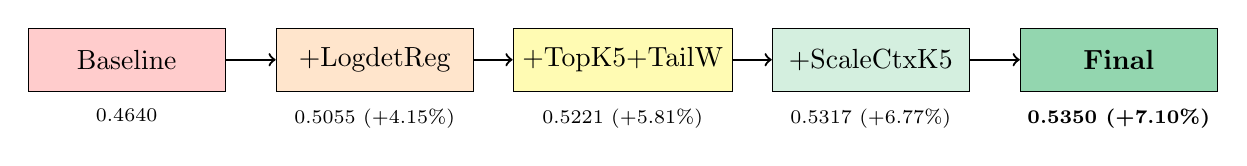
\begin{tikzpicture}[scale=0.9]
    % Baseline
    \node[draw, fill=red!20, minimum width=2.5cm, minimum height=0.8cm] (b) at (0,0) {Baseline};
    \node[below=0.1cm of b] {\scriptsize 0.4640};

    % +LogdetReg
    \node[draw, fill=orange!20, minimum width=2.5cm, minimum height=0.8cm] (l) at (3.5,0) {+LogdetReg};
    \node[below=0.1cm of l] {\scriptsize 0.5055 (+4.15\%)};

    % +TopK5+TailW
    \node[draw, fill=yellow!30, minimum width=2.5cm, minimum height=0.8cm] (t) at (7,0) {+TopK5+TailW};
    \node[below=0.1cm of t] {\scriptsize 0.5221 (+5.81\%)};

    % +ScaleCtxK5
    \node[draw, fill=accentgreen!20, minimum width=2.5cm, minimum height=0.8cm] (s) at (10.5,0) {+ScaleCtxK5};
    \node[below=0.1cm of s] {\scriptsize 0.5317 (+6.77\%)};

    % Final
    \node[draw, fill=accentgreen!50, minimum width=2.5cm, minimum height=0.8cm] (f) at (14,0) {\textbf{Final}};
    \node[below=0.1cm of f] {\scriptsize \textbf{0.5350 (+7.10\%)}};

    % Arrows
    \draw[->, thick] (b) -- (l);
    \draw[->, thick] (l) -- (t);
    \draw[->, thick] (t) -- (s);
    \draw[->, thick] (s) -- (f);
\end{tikzpicture}
\end{center}

\vspace{1em}
\textbf{최적 설정:}
\begin{itemize}
    \item \texttt{TailW=0.55, TopK=5, LogdetReg=1e-4, ScaleCtxK=5, lr=3e-4}
\end{itemize}
\end{frame}

%-------------------------------------------------------------------------------
% Frame: Component Importance Analysis (MoLE6+DIA2 Baseline)
%-------------------------------------------------------------------------------
\begin{frame}{Component Importance Analysis (MoLE6+DIA2 기준)}
\textbf{Ablation Study: 컴포넌트별 Pix AP 기여도 순위}

\begin{table}
\centering
\scriptsize
\begin{tabular}{lcccc}
\toprule
\textbf{Component} & \textbf{w/o Pix AP} & \textbf{MAIN (56.18)} & \textbf{기여도} & \textbf{Impact} \\
\midrule
\textcolor{red}{\textbf{Tail Aware Loss}} & 48.61 & 56.18 & \textcolor{red}{\textbf{+7.57\%p}} & \ding{72}\ding{72}\ding{72}\ding{72}\ding{72} \\
\textbf{Whitening Adapter} & 48.84 & 56.18 & \textcolor{red}{\textbf{+7.34\%p}} & \ding{72}\ding{72}\ding{72}\ding{72}\ding{72} \\
LogDet Regularization & 51.85 & 56.18 & +4.33\%p & \ding{72}\ding{72}\ding{72}\ding{72} \\
Spatial Context & 52.93 & 56.18 & +3.25\%p & \ding{72}\ding{72}\ding{72} \\
Pos Embedding & 53.99 & 56.18 & +2.19\%p & \ding{72}\ding{72} \\
Scale Context & 54.52 & 56.18 & +1.66\%p & \ding{72}\ding{72} \\
LoRA & 55.31 & 56.18 & +0.87\%p & \ding{72} \\
\bottomrule
\end{tabular}
\end{table}

\vspace{0.3em}
\begin{columns}
\begin{column}{0.48\textwidth}
\textbf{핵심 발견:}
\begin{enumerate}
    \item \textbf{Tail Aware Loss}: 단일 최대 개선 (+7.57\%p)
    \item \textbf{Whitening Adapter}: 두 번째로 중요 (+7.34\%p)
    \item \textbf{LoRA}: 기여도 낮음 (DIA가 역할 분담)
\end{enumerate}
\end{column}
\begin{column}{0.48\textwidth}
\textbf{주의사항:}
\begin{itemize}
    \item MoLE$\geq$12: 학습 불안정
    \item spatial\_ctx\_k$\geq$5: Pix AP 급락
    \item tail\_weight$>$1.0: 역효과
\end{itemize}
\end{column}
\end{columns}
\end{frame}

%-------------------------------------------------------------------------------
% Frame: Key Trade-offs Discovered
%-------------------------------------------------------------------------------
\begin{frame}{Key Trade-offs Discovered}
\textbf{실험을 통해 발견된 핵심 Trade-off:}

\vspace{0.5em}
\begin{columns}
\begin{column}{0.48\textwidth}
\textbf{1. DIA Blocks vs Pixel AP}
\begin{table}
\scriptsize
\begin{tabular}{ccc}
\toprule
DIA Blocks & Image AUC & Pixel AP \\
\midrule
2 (MAIN) & 0.9792 & \textbf{0.5618} \\
4 & 0.9793 & 0.4735 \\
6 & 0.9820 & 0.4606 \\
8 & \textbf{0.9825} & 0.4546 \\
\bottomrule
\end{tabular}
\end{table}
$\uparrow$ DIA $\rightarrow$ $\uparrow$ Image AUC, $\downarrow$ Pixel AP
\end{column}

\begin{column}{0.48\textwidth}
\textbf{2. TailWeight vs Stability}
\begin{table}
\scriptsize
\begin{tabular}{ccc}
\toprule
TailW & Image AUC & Pixel AP \\
\midrule
0.50 & \textbf{0.983} & 0.5221 \\
\textbf{0.70 (MAIN)} & 0.9792 & \textbf{0.5618} \\
0.80 & 0.981 & 0.5447 \\
\bottomrule
\end{tabular}
\end{table}
$\uparrow$ TailW $\rightarrow$ $\uparrow$ Pixel AP (최적: 0.70)
\end{column}
\end{columns}

\vspace{0.5em}
\begin{alertblock}{최적 균형점 (MoLE6+DIA2)}
\textbf{권장 설정}: MoLE=6, DIA=2, TailW=0.70, TopK=3, LogdetReg=1e-4 \\
$\rightarrow$ Image AUC \textbf{97.92\%}, Pixel AUC \textbf{97.81\%}, Pixel AP \textbf{55.80\%}
\end{alertblock}
\end{frame}

%-------------------------------------------------------------------------------
% Frame: Top 10 Experiments by Pixel AP
%-------------------------------------------------------------------------------
\begin{frame}{Top 10 Experiments by Pixel AP}
\begin{table}
\centering
\scriptsize
\begin{tabular}{clccc}
\toprule
\textbf{Rank} & \textbf{Configuration} & \textbf{Image AUC} & \textbf{Pixel AP} & \textbf{Routing} \\
\midrule
1 & TailW0.55-TopK5-LogdetReg1e-4-ScaleCtxK5-lr3e-4 & 0.9824 & \textbf{0.5350} & 100\% \\
2 & TailW0.65-TailTopK3-TopK5-LogdetReg1e-4 & 0.9827 & 0.5324 & 100\% \\
3 & TopK3-TailW0.5-LogdetReg1e-4-ScaleCtxK5 & 0.9802 & 0.5317 & 100\% \\
4 & TopK5-TailW0.5-LogdetReg1e-4-ScaleCtxK5 & 0.9809 & 0.5317 & 100\% \\
5 & TailW0.6-TailTopK3-TopK5-LogdetReg1e-4-ScaleCtxK5-80ep & 0.9826 & 0.5310 & 100\% \\
6 & TailW0.6-TopK5-LogdetReg1e-4 & 0.9827 & 0.5290 & 100\% \\
7 & TailW0.55-TopK5-LogdetReg1e-4 & 0.9827 & 0.5256 & 100\% \\
8 & TailW0.5-TailTopK3-TopK5-LogdetReg1e-4 & 0.9830 & 0.5242 & 100\% \\
9 & FullBest-80ep-lr3e-4-LoRA128-C10-DIA5-TailW0.55 & \textbf{0.9836} & 0.5242 & 100\% \\
10 & TopK5-TailW0.5-LogdetReg1e-4 & 0.9826 & 0.5221 & 100\% \\
\bottomrule
\end{tabular}
\end{table}

\vspace{0.5em}
\textbf{Observation:} 모든 상위 설정에서 \textbf{Routing Accuracy 100\%} 유지
\end{frame}

%-------------------------------------------------------------------------------
% Frame: Per-Class Performance Improvement
%-------------------------------------------------------------------------------
\begin{frame}{Per-Class Performance Improvement}
\begin{table}
\centering
\scriptsize
\begin{tabular}{lccc}
\toprule
\textbf{Class} & \textbf{Baseline} & \textbf{Top Config} & \textbf{Improvement} \\
\midrule
carpet & 0.3601 & 0.6167 & \textcolor{accentgreen}{\textbf{+0.2566}} \\
bottle & 0.4551 & 0.6774 & \textcolor{accentgreen}{\textbf{+0.2223}} \\
leather & 0.2292 & 0.3970 & \textcolor{accentgreen}{\textbf{+0.1678}} \\
toothbrush & 0.4028 & 0.5619 & +0.1591 \\
wood & 0.3546 & 0.4453 & +0.0907 \\
hazelnut & 0.5110 & 0.5798 & +0.0688 \\
\midrule
metal\_nut & 0.8491 & 0.7776 & \textcolor{red}{-0.0715} \\
cable & 0.6575 & 0.6339 & \textcolor{red}{-0.0236} \\
\midrule
\textbf{Mean} & \textbf{0.4640} & \textbf{0.5350} & \textbf{+0.0710} \\
\bottomrule
\end{tabular}
\end{table}

\textbf{Key Observations:}
\begin{itemize}
    \item \textcolor{accentgreen}{\textbf{Textured classes}} (carpet, leather): 가장 큰 개선
    \item \textcolor{red}{\textbf{Fine-grained objects}} (metal\_nut, cable): 약간의 성능 저하
\end{itemize}
\end{frame}

%-------------------------------------------------------------------------------
% Frame: Hyperparameter Sensitivity Summary - UPDATED 2026-01-08
%-------------------------------------------------------------------------------
\begin{frame}{Hyperparameter Sensitivity Summary (MoLE6+DIA2 기준)}
\begin{columns}
\begin{column}{0.5\textwidth}
\textbf{lambda\_logdet (Critical)}
\begin{table}
\scriptsize
\begin{tabular}{ccc}
\toprule
$\lambda_{\text{logdet}}$ & Img AUC & Pix AP \\
\midrule
0 (disabled) & 98.06 & 51.85 \\
1e-6 & 98.08 & 51.88 \\
1e-5 & 98.10 & 52.46 \\
\textbf{1e-4} & 97.92 & \textbf{56.18} \\
\bottomrule
\end{tabular}
\end{table}
\begin{itemize}
    \item \textbf{1e-4}가 최적 (+4.30\%p)
    \item 1e-6/1e-5는 효과 미미
\end{itemize}
\end{column}

\begin{column}{0.5\textwidth}
\textbf{spatial\_context\_kernel (\textcolor{red}{Critical})}
\begin{table}
\scriptsize
\begin{tabular}{ccc}
\toprule
Kernel & Img AUC & Pix AP \\
\midrule
0 (disabled) & 97.98 & 52.93 \\
\textbf{3} & \textbf{97.92} & \textbf{56.18} \\
5 & 96.12 & 51.38 \\
7 & 90.90 & 44.33 \\
\bottomrule
\end{tabular}
\end{table}
\begin{itemize}
    \item \textbf{Kernel=3}이 최적
    \item Kernel$\geq$5에서 \textcolor{red}{\textbf{급락}}
\end{itemize}
\end{column}
\end{columns}

\vspace{0.5em}
\begin{alertblock}{Warning: Spatial Context Kernel}
\textbf{kernel=5}: Pix AP -4.80\%p, \textbf{kernel=7}: Pix AP \textcolor{red}{\textbf{-11.85\%p}} (학습 불안정)
\end{alertblock}
\end{frame}

%-------------------------------------------------------------------------------
% Frame: Optimal Configuration Recommendations - UPDATED 2026-01-08
%-------------------------------------------------------------------------------
\begin{frame}{Optimal Configuration (MoLE6+DIA2)}
\begin{columns}
\begin{column}{0.5\textwidth}
\textbf{Recommended Setting (최고 Pix AP)}
\begin{itemize}
    \item \texttt{num\_coupling\_layers = 6}
    \item \texttt{dia\_n\_blocks = 2}
    \item \texttt{tail\_weight = 1.0}
    \item \texttt{tail\_top\_k\_ratio = 0.02}
    \item \texttt{lambda\_logdet = 1e-4}
    \item \texttt{scale\_context\_kernel = 5}
    \item \texttt{spatial\_context\_kernel = 3}
    \item \texttt{lora\_rank = 64}
    \item \texttt{lr = 3e-4}
    \item \texttt{epochs = 60}
\end{itemize}
\end{column}

\begin{column}{0.5\textwidth}
\textbf{Expected Performance}
\begin{table}
\begin{tabular}{lc}
\toprule
\textbf{Metric} & \textbf{Value} \\
\midrule
Image AUC & 97.92\% \\
Pixel AUC & 97.81\% \\
Pixel AP & \textbf{56.18\%} \\
Routing Acc. & 100\% \\
\bottomrule
\end{tabular}
\end{table}

\vspace{0.5em}
\textbf{주의사항}
\begin{itemize}
    \item spatial\_ctx\_k $\neq$ 3 금지
    \item tail\_weight $>$ 1.0 비권장
    \item MoLE $\geq$ 12 학습 불안정
\end{itemize}
\end{column}
\end{columns}
\end{frame}

%===============================================================================
\section{Experiments Part 2: Paper Experiment Design}
%===============================================================================

%-------------------------------------------------------------------------------
% Frame: Experimental Setup
%-------------------------------------------------------------------------------
\begin{frame}{Experimental Setup}
\begin{columns}
\begin{column}{0.5\textwidth}
\textbf{Datasets}
\begin{itemize}
    \item \textbf{MVTec AD}: 15 classes, 5,354 images
    \item \textbf{VisA}: 12 classes, 10,821 images
    \item \textbf{MPDD}: 6 classes (metal parts)
\end{itemize}

\vspace{0.5em}
\textbf{Evaluation Metrics}
\begin{itemize}
    \item Image AUROC / AP (primary)
    \item Pixel AUROC / AP / PRO
    \item Forgetting (F), BWT
    \item Routing Accuracy
\end{itemize}
\end{column}

\begin{column}{0.5\textwidth}
\textbf{Implementation}
\begin{itemize}
    \item Backbone: ViT-Base-16 (frozen)
    \item NF: 8 Coupling Layers
    \item LoRA rank: 64
    \item DIA: 4 blocks
    \item Epochs: 60 per task
    \item LR: $2 \times 10^{-4}$
    \item Input: 224 $\times$ 224
\end{itemize}

\vspace{0.5em}
\textbf{Hardware}: NVIDIA RTX 4090
\end{column}
\end{columns}
\end{frame}

%-------------------------------------------------------------------------------
% Frame: Continual Learning Scenarios
%-------------------------------------------------------------------------------
\begin{frame}{Continual Learning Scenarios}
\textbf{4가지 시나리오로 지속 학습 능력 검증:}

\vspace{0.5em}
\begin{enumerate}
    \item \textbf{Scenario A: Standard 5-Task Protocol}
    \begin{itemize}
        \item MVTec 15 classes $\rightarrow$ 5 tasks (각 3 classes)
        \item Task 0: leather, grid, transistor (텍스처 + 객체 혼합)
    \end{itemize}

    \vspace{0.3em}
    \item \textbf{Scenario B: Long Sequence (15-Task)}
    \begin{itemize}
        \item 15개 클래스를 각각 독립 작업으로 구성
        \item 장기 망각(Long-term Forgetting) 분석
    \end{itemize}

    \vspace{0.3em}
    \item \textbf{Scenario C: Class Order Sensitivity}
    \begin{itemize}
        \item 5개 무작위 순서로 학습
        \item Parameter Isolation의 순서 견고성 검증
    \end{itemize}

    \vspace{0.3em}
    \item \textbf{Scenario D: Task 0 Dependency Analysis}
    \begin{itemize}
        \item Texture-first vs Object-first vs Mixed-first
        \item Base weights 학습이 후속 작업에 미치는 영향
    \end{itemize}
\end{enumerate}
\end{frame}

%-------------------------------------------------------------------------------
% Frame: Comparison with SOTA Methods
%-------------------------------------------------------------------------------
\begin{frame}{Comparison with SOTA Methods}
\textbf{비교 대상:}

\vspace{0.5em}
\begin{columns}
\begin{column}{0.5\textwidth}
\textbf{Continual AD Methods}
\begin{itemize}
    \item \textbf{DNE}: 분포 저장 기반
    \item \textbf{UCAD}: Prompt tuning 기반 SOTA
\end{itemize}

\vspace{0.5em}
\textbf{CL + AD Adaptation}
\begin{itemize}
    \item EWC: 중요 파라미터 정규화
    \item LwF: Knowledge Distillation
    \item Replay (5\%): 데이터 저장
\end{itemize}
\end{column}

\begin{column}{0.5\textwidth}
\textbf{Bounds}
\begin{itemize}
    \item \textbf{Joint Training}: Upper bound
    \item \textbf{Task-Separated}: 망각 없음, 비효율
    \item \textbf{Fine-tuning}: Lower bound
\end{itemize}

\vspace{0.5em}
\textbf{검증 목표:}
\begin{itemize}
    \item 이상 탐지 성능 우수성
    \item Forgetting $\approx$ 0 (Parameter Isolation)
    \item Routing Accuracy 100\%
\end{itemize}
\end{column}
\end{columns}
\end{frame}

%-------------------------------------------------------------------------------
% Frame: Ablation Study Design (7 Components) - UPDATED 2026-01-08
%-------------------------------------------------------------------------------
\begin{frame}{Ablation Study: 컴포넌트별 중요도 분석 (MoLE6+DIA2 기준)}
\begin{table}
\centering
\scriptsize
\begin{tabular}{lccccl}
\toprule
\textbf{Configuration} & \textbf{Img AUC} & \textbf{Pix AUC} & \textbf{Pix AP} & \textbf{$\Delta$ Pix AP} & \textbf{Importance} \\
\midrule
\textbf{MAIN (MoLE6+DIA2)} & \textbf{97.92} & \textbf{97.81} & \textbf{56.18} & - & Baseline \\
\midrule
\multicolumn{6}{l}{\textit{Loss Components (가장 중요)}} \\
\quad w/o Tail Aware Loss & 94.97 & 97.21 & 48.61 & \textcolor{red}{\textbf{-7.57}} & \ding{72}\ding{72}\ding{72}\ding{72}\ding{72} \\
\midrule
\multicolumn{6}{l}{\textit{Core Adapters}} \\
\quad w/o Whitening Adapter & 97.90 & 97.69 & 48.84 & \textcolor{red}{\textbf{-7.34}} & \ding{72}\ding{72}\ding{72}\ding{72}\ding{72} \\
\quad w/o LogDet Reg & 98.06 & 97.70 & 51.85 & \textcolor{red}{-4.33} & \ding{72}\ding{72}\ding{72}\ding{72} \\
\quad w/o LoRA & 97.96 & 97.77 & 55.31 & -0.87 & \ding{72} \\
\midrule
\multicolumn{6}{l}{\textit{Context Modules}} \\
\quad w/o Spatial Context & 97.98 & 97.54 & 52.93 & \textcolor{red}{-3.25} & \ding{72}\ding{72}\ding{72} \\
\quad w/o Pos Embedding & 97.40 & 97.47 & 53.99 & -2.19 & \ding{72}\ding{72} \\
\quad w/o Scale Context & 97.90 & 97.74 & 54.52 & -1.66 & \ding{72}\ding{72} \\
\bottomrule
\end{tabular}
\end{table}

\begin{alertblock}{Key Insight}
\textbf{Tail Aware Loss} (+7.57\%p)와 \textbf{Whitening Adapter} (+7.34\%p)가 Pix AP에 가장 중요
\end{alertblock}
\end{frame}

%-------------------------------------------------------------------------------
% Frame: Training Strategy Ablation - NEW
%-------------------------------------------------------------------------------
\begin{frame}{Training Strategy: Base Freezing의 중요성}
\textbf{Base Weights Freeze vs Sequential Training}

\begin{table}
\centering
\begin{tabular}{lcccc}
\toprule
\textbf{Strategy} & \textbf{Img AUC} & \textbf{Pix AP} & \textbf{$\Delta$ Img AUC} & \textbf{$\Delta$ Pix AP} \\
\midrule
\textbf{MAIN (Base Frozen)} & \textbf{97.92\%} & \textbf{56.18\%} & - & - \\
Sequential Training & 60.10\% & 12.29\% & \textcolor{red}{\textbf{-37.82\%}} & \textcolor{red}{\textbf{-43.89\%}} \\
Complete Separated & 98.13\% & 52.49\% & +0.21\% & -3.69\% \\
\bottomrule
\end{tabular}
\end{table}

\vspace{0.5em}
\textbf{분석:}
\begin{itemize}
    \item \textbf{Sequential Training}: Base freeze 없이 순차 학습 $\rightarrow$ \textcolor{red}{\textbf{Catastrophic Forgetting 발생}}
    \item \textbf{Complete Separated}: 공유 weight 없이 완전 분리 $\rightarrow$ 공유 representation 학습 이점 상실
    \item \textbf{Base Frozen (Ours)}: Parameter Isolation으로 Forgetting 방지 + 공유 학습 이점 유지
\end{itemize}

\begin{alertblock}{핵심 결론}
Base Frozen 전략이 Continual Learning에 \textbf{필수}: Sequential 대비 Img AUC +37.82\%p
\end{alertblock}
\end{frame}

%-------------------------------------------------------------------------------
% Frame: MoLE vs DIA Architecture Comparison - NEW
%-------------------------------------------------------------------------------
\begin{frame}{Architecture Comparison: MoLE vs DIA}
\begin{table}
\centering
\scriptsize
\begin{tabular}{lcccccl}
\toprule
\textbf{Architecture} & \textbf{MoLE} & \textbf{DIA} & \textbf{Total} & \textbf{Img AUC} & \textbf{Pix AP} & \textbf{Note} \\
\midrule
\textbf{MoLE+DIA} & \textbf{6} & \textbf{2} & \textbf{8} & \textbf{97.92} & \textbf{56.18} & \textcolor{accentgreen}{\textbf{최적}} \\
MoLE+DIA & 4 & 2 & 6 & 97.84 & 55.90 & \\
MoLE+DIA & 8 & 2 & 10 & 97.99 & 54.92 & \\
MoLE+DIA & 8 & 4 & 12 & 98.29 & 54.20 & Old MAIN \\
\midrule
DIA-Only & 0 & 4 & 4 & 98.13 & 53.28 & 안정적 \\
DIA-Only & 0 & 8 & 8 & 98.19 & 50.74 & \\
\midrule
MoLE-Only & 8 & 0 & 8 & 92.74 & 50.06 & \textcolor{red}{불안정} \\
MoLE-Only & 12 & 0 & 12 & 62.19 & 14.23 & \textcolor{red}{학습 실패} \\
\bottomrule
\end{tabular}
\end{table}

\begin{alertblock}{핵심 발견}
\begin{itemize}
    \item \textbf{MoLE-Only}: DIA 없이는 Img AUC 92.74\%로 \textbf{-5.18\%p 하락}, depth$\geq$12에서 학습 실패
    \item \textbf{DIA-Only}: 안정적이나 Pix AP 53.28\%로 제한적 (-2.90\%p)
    \item \textbf{MoLE+DIA}: DIA가 MoLE 학습 안정화 $\rightarrow$ 안정성 + 정밀도 모두 달성
\end{itemize}
\end{alertblock}
\end{frame}

%-------------------------------------------------------------------------------
% Frame: Cross-Dataset Generalization
%-------------------------------------------------------------------------------
\begin{frame}{Cross-Dataset Generalization}
\textbf{MVTec $\rightarrow$ VisA $\rightarrow$ MPDD 일반화 평가:}

\begin{table}
\centering
\begin{tabular}{lcccc}
\toprule
\textbf{Dataset} & \textbf{Classes} & \textbf{Image AUC} & \textbf{Pixel AP} & \textbf{Routing Acc.} \\
\midrule
MVTec AD & 15 & \textbf{0.9824} & \textbf{0.5350} & 100\% \\
VisA & 12 & 0.8566 & 0.2878 & 100\% \\
MPDD & 6 & 0.9019 & 0.2890 & 98.12\% \\
\bottomrule
\end{tabular}
\end{table}

\vspace{0.5em}
\textbf{VisA Analysis:}
\begin{itemize}
    \item 복잡한 텍스처와 미세 결함 $\rightarrow$ 더 도전적
    \item 병목 클래스: macaroni1/2 (Pixel AP $<$ 0.1)
    \item ViT backbone: Image AUC 0.88 (WRN50 대비 +4.2\%)
\end{itemize}

\textbf{MPDD:}
\begin{itemize}
    \item 금속 표면의 유사성 $\rightarrow$ Routing 오류 (98.12\%)
\end{itemize}
\end{frame}

%-------------------------------------------------------------------------------
% Frame: Continual Learning Analysis
%-------------------------------------------------------------------------------
\begin{frame}{Continual Learning Analysis}
\textbf{Forgetting 분석:}
\begin{itemize}
    \item Parameter Isolation (LoRA + DIA) $\rightarrow$ \textbf{Forgetting $\approx$ 0}
    \item vs Fine-tuning: 급격한 성능 하락
    \item vs EWC/LwF: 완만한 하락
\end{itemize}

\vspace{1em}
\textbf{Router Performance:}
\begin{itemize}
    \item 5-Task: 100\% Routing Accuracy
    \item 15-Task: Oracle과의 Gap 분석
    \item Task 수 증가에 따른 Scalability 검증
\end{itemize}

\vspace{1em}
\textbf{Storage Efficiency:}
\begin{itemize}
    \item MoLE-Flow: 약 2MB/Task (LoRA + DIA)
    \item vs Replay (5\%): 50MB/Task $\rightarrow$ \textbf{25x 절약}
\end{itemize}
\end{frame}

%===============================================================================
\section{Conclusion \& Future Work}
%===============================================================================

%-------------------------------------------------------------------------------
% Frame: Summary - UPDATED 2026-01-08
%-------------------------------------------------------------------------------
\begin{frame}{Summary: Key Findings}
\textbf{MoLE-Flow 최종 성능 (MVTec AD, 15 classes)}

\begin{center}
\begin{tabular}{lccc}
\toprule
\textbf{Metric} & \textbf{Value} & \textbf{비고} \\
\midrule
Image AUC & 97.92\% & MoLE6+DIA2 \\
Pixel AUC & 97.81\% & \\
Pixel AP & \textbf{56.18\%} & \\
Routing Accuracy & 100\% & \\
\bottomrule
\end{tabular}
\end{center}

\vspace{0.5em}
\textbf{핵심 발견사항:}
\begin{enumerate}
    \item \textbf{가장 중요한 컴포넌트}: Tail Aware Loss (+7.57\%p), Whitening Adapter (+7.34\%p)
    \item \textbf{가장 민감한 하이퍼파라미터}: spatial\_context\_kernel (kernel$\geq$5에서 급락)
    \item \textbf{최적 아키텍처}: MoLE=6, DIA=2 (총 8 blocks)
    \item \textbf{Parameter Isolation 효과}: Sequential Training 대비 +37.82\%p Img AUC
\end{enumerate}

\begin{alertblock}{결론}
Parameter Isolation (LoRA + DIA) + Tail-Aware Loss + Whitening Adapter가 \\
Continual Anomaly Detection에서 최적 성능 달성
\end{alertblock}
\end{frame}

%-------------------------------------------------------------------------------
% Frame: Key Results - UPDATED 2026-01-08
%-------------------------------------------------------------------------------
\begin{frame}{Key Results (MoLE6+DIA2 Configuration)}
\begin{columns}
\begin{column}{0.5\textwidth}
\textbf{MVTec AD (15 classes, 1x1 CL)}
\begin{itemize}
    \item Image AUC: \textbf{97.92\%}
    \item Pixel AUC: \textbf{97.81\%}
    \item Pixel AP: \textbf{56.18\%}
    \item Routing Acc.: \textbf{100\%}
\end{itemize}

\vspace{0.5em}
\textbf{컴포넌트 기여도 (Pix AP 기준)}
\begin{enumerate}
    \item Tail Aware Loss: \textbf{+7.57\%p}
    \item Whitening Adapter: \textbf{+7.34\%p}
    \item LogDet Reg: +4.33\%p
    \item Spatial Context: +3.25\%p
\end{enumerate}
\end{column}

\begin{column}{0.5\textwidth}
\textbf{핵심 하이퍼파라미터}
\begin{table}
\scriptsize
\begin{tabular}{lcc}
\toprule
\textbf{Parameter} & \textbf{최적값} & \textbf{민감도} \\
\midrule
tail\_weight & 1.0 & \textcolor{red}{높음} \\
lambda\_logdet & 1e-4 & \textcolor{red}{높음} \\
spatial\_ctx\_k & 3 & \textcolor{red}{높음} \\
scale\_ctx\_k & 5 & 중간 \\
lora\_rank & 16-64 & 낮음 \\
\bottomrule
\end{tabular}
\end{table}

\vspace{0.3em}
\textbf{Warning}
\begin{itemize}
    \item spatial\_ctx\_k $\geq$ 5: 성능 급락
    \item tail\_weight $>$ 1.0: 역효과
\end{itemize}
\end{column}
\end{columns}
\end{frame}

%-------------------------------------------------------------------------------
% Frame: Future Work
%-------------------------------------------------------------------------------
\begin{frame}{Future Work}
\textbf{1. 성능 향상 방향}
\begin{itemize}
    \item Pixel AP 0.6+ 달성을 위한 추가 최적화
    \item 고해상도 입력 (448 $\times$ 448) 적용
    \item DINOv2 ViT-L/H 등 강력한 backbone 탐색
\end{itemize}

\vspace{1em}
\textbf{2. 일반화 강화}
\begin{itemize}
    \item VisA 병목 클래스 (macaroni) 특화 전략
    \item Multi-scale 평가 앙상블
    \item Class-specific hyperparameter tuning
\end{itemize}

\vspace{1em}
\textbf{3. 실용화 연구}
\begin{itemize}
    \item 실시간 추론 최적화
    \item 경량화 (Quantization, Pruning)
    \item 온라인 학습 시나리오 확장
\end{itemize}
\end{frame}

%-------------------------------------------------------------------------------
% Frame: Thank You
%-------------------------------------------------------------------------------
\begin{frame}
\centering
\Huge Thank You!

\vspace{2em}
\Large Questions?

\vspace{3em}
\normalsize
\textbf{GitHub}: \texttt{github.com/your-repo/moleflow}

\textbf{Contact}: author@example.com
\end{frame}

\end{document}
